\batchmode
\documentclass[11pt,a4paper]{book}
\RequirePackage{ifthen}


\usepackage{ujthesis,float,enumerate,amssymb,amsmath,algorithm,algpseudocode}
\usepackage{cite,graphicx,tikz,xcolor,appendix,hyperref}
\usepackage[acronym,toc]{glossaries}
\usetikzlibrary{plothandlers}
\usetikzlibrary{positioning}
\usetikzlibrary{decorations.pathreplacing}
\usetikzlibrary{patterns}
\usetikzlibrary{shapes.geometric}
\usetikzlibrary{shapes.symbols}
\usetikzlibrary{shapes.misc}
\raggedbottom
\usepackage[nottoc]{tocbibind}
\linespread{1.2}
\dissertation
\coverFont{\large }

\setlength{\parskip}{0.5ex plus0.5ex minus0.2ex} 

\setlength{\ Length}{7mm} 
\approvedtitle{Optimising the Frequency Assignment Problem utilizing Particle Swarm Optimisation}
\student{William Bezuidenhout}
\degree{Magister Scientiae}
\field{Information Technology}
\faculty{Faculty of Science}
\supervisorName{Dr G.B. O'Reilly}
\submissionDate{May 2012}
\makeglossaries
\newacronym{FAP}{FAP}{frequency assignment problem}
\newacronym{gsm}{GSM}{general system for mobile communication}
\newacronym{SMS}{SMS}{short message service}
\newacronym{MMS}{MMS}{multimedia message service}
\newacronym{GPRS}{GPRS}{general packet radio system}
\newacronym{EDGE}{EDGE}{enhanced data global evolution}
\newacronym{HSCSD}{HSCSD}{high speed circuit switched data}
\newacronym{ISDN}{ISDN}{integrated service digital network}
\newacronym{DCS1800}{DCS1800}{digital cellular system}
\newacronym{TDMA}{TDMA}{time division multiple access}
\newacronym{SIR}{SIR}{signal-to-noise ratio}
\newacronym{UMTS}{UMTS}{universal mobile telecommunications system}
\newacronym{DS-CDMA}{DS-CDMA}{direct sequence collision detection multiple access}
\newacronym{WCDMA}{WCDMA}{wide band collision detection multiple access}
\newacronym{CDMA}{CDMA}{code division multiple access}
\newacronym{LTE}{LTE}{long term evolution}
\newacronym{WIMAX}{WiMAX}{worlwide interoperability for microwave access}
\newacronym{MS}{MS}{mobile station}
\newacronym{POS}{POS}{[point of sale}
\newacronym{SIM}{SIM}{subscriber identification module}
\newacronym{IMSI}{IMSI}{international mobile subscriber identity}
\newacronym{IMEI}{IMEI}{international mobile equipment identity}
\newacronym{BTS}{BTS}{base tranceiver stations}
\newacronym{MSC}{MSC}{mobile switching centre}
\newacronym{BSS}{BSS}{base station subsystem}
\newacronym{BSC}{BSC}{base station controller}
\newacronym{LA}{LA}{location area}
\newacronym{TRX}{TRX}{transceiver}
\newacronym{TDM}{TDM}{time division multiplexing}
\newacronym{FDM}{FDM}{frequency division multiplexing}
\newacronym{NSS}{NSS}{network switching subsystem}
\newacronym{VLR}{VLR}{visitor location register}
\newacronym{HLR}{HLR}{home location register}
\newacronym{PSTN}{PSTN}{public switching telephone network}
\newacronym{AUC}{AUC}{authentication centre}
\newacronym{EIR}{EIR}{equipment identity register}
\newacronym{SRES}{SRES}{signed response}
\newacronym{OMC}{OMC}{operations and management centre}
\newacronym{NMC}{NMC}{network management centre}
\newacronym{LAPDm}{LAPDm}{link access protocol D channel modified}
\newacronym{TCH}{TCH}{traffic channel}
\newacronym{BCH}{BCH}{broadcast channel}
\newacronym{CCCH}{CCCH}{common control channel}
\newacronym{DCCH}{DCCH}{dedicated control channel}
\newacronym{BCCH}{BCCH}{broadcast control channel}
\newacronym{FCCH}{FCCH}{frequency control channel}
\newacronym{SCH}{SCH}{sychronisation channel}
\newacronym{RACH}{RACH}{random access channel}
\newacronym{AGCH}{AGCH}{access grant channel}
\newacronym{PCH}{PCH}{paging channel}
\newacronym{NCH}{NCH}{notification channel}
\newacronym{D/ACCH}{D/ACCH}{dedicated/associated control channel}
\newacronym{SDCCH}{SDCCH}{stand-alone dedicated control channel}
\newacronym{SACCH}{SACCH}{slow associated control channel}
\newacronym{FACCH}{FACCH}{fast associated control channel}
\newacronym{CBCH}{CBCH}{cell broadcast control channel}
\newacronym{AFP}{AFP}{automatic frequency planning}
\newacronym{CAP}{CAP}{channel assignment problem}
\newacronym{FFA}{FFA}{fixed frequency allocation}
\newacronym{FCA}{FCA}{fixed channel allocation}
\newacronym{DFA}{DFA}{dynamic frequency allocation}
\newacronym{DCA}{DCA}{dynamic channel allocation}
\newacronym{QoS}{QoS}{quality of service}
\newacronym{SINR}{SINR}{signal to interference noise power ration}
\newacronym{BER}{BER}{bit error rate}
\newacronym{MO-FAP}{MO-FAP}{minimum-order frequency assignment problem}
\newacronym{MS-FAP}{MS-FAP}{minimum span frequency assignment problem}
\newacronym{MI-FAP}{MI-FAP}{minimum interference frequency assignment problem}
\newacronym{FS-FAP}{FS-FAP}{fixed spectrum frequency assignment problem}
\newacronym{EUCLID}{EUCLID}{EUropean Cooperation on the Long term in the Defense}
\newacronym{CELAR}{CELAR}{cenre d'electronique de l'armement}
\newacronym{COST}{COST}{COop\'{e}ration europ\'{e}ene dans le domaine de la recherche Scientifique et Technique}
\newacronym{WLAN}{WLAN}{wireless local area network}
\newacronym{AP}{AP}{access point}
\newacronym{SA}{SA}{simulated annealing}
\newacronym{AI}{AI}{artificial intelligence}
\newacronym{TS}{TS}{tabu search}
\newacronym{MTM}{MTM}{medium term memory}
\newacronym{LTM}{LTM}{long term memory}
\newacronym{STM}{STM}{short term memory}
\newacronym{HMT}{HMT}{heuristic manipulation technique}
\newacronym{GA}{GA}{genetic algorithm}
\newacronym{CGA}{CGA}{canical genetic algorithm}
\newacronym{PRNG}{PRNG}{pseudo random number generator}
\newacronym{QRNG}{QRNG}{quasi random number generator}
\newacronym{ACO}{ACO}{ant colony optimisation}
\newacronym{PSO}{PSO}{particle swarm optimisation}
\newacronym{ABC}{ABC}{artificial bee colony}
\newacronym{SACO}{SACO}{simple ant colony optimisation}
\newacronym{AS}{AS}{ant system}
\newacronym{ACS}{ACS}{ant colony system}
\newacronym{ANTS}{ANTS}{approximate non-deterministic tree search}
\newacronym{BCO}{BCO}{bee colony optimisation}
\newacronym{BSO}{BSO}{bee swarm optimisation}
\newacronym{VBA}{VBA}{virtual bee algorithm}
\newacronym{ARPSO}{ARPSO}{attract repulse particle swarm optimisation}
\newacronym{FEA}{FEA}{frequency exhaustive assignment}
\newacronym{MMAS}{MMAS}{min-max ant system}


\usepackage[dvips]{color}


\pagecolor[gray]{.7}

\usepackage[latin1]{inputenc}



\makeatletter
\AtBeginDocument{\makeatletter
\input /Users/william/Dropbox/Masters/Dissertation/dissertation.aux
\makeatother
}
\AtBeginDocument{\makeatletter
\input /Users/william/Dropbox/Masters/Dissertation/chpt1.aux
\makeatother
}
\AtBeginDocument{\makeatletter
\input /Users/william/Dropbox/Masters/Dissertation/chpt2.aux
\makeatother
}
\AtBeginDocument{\makeatletter
\input /Users/william/Dropbox/Masters/Dissertation/chpt3.aux
\makeatother
}
\AtBeginDocument{\makeatletter
\input /Users/william/Dropbox/Masters/Dissertation/chpt4.aux
\makeatother
}
\AtBeginDocument{\makeatletter
\input /Users/william/Dropbox/Masters/Dissertation/chpt5.aux
\makeatother
}
\AtBeginDocument{\makeatletter
\input /Users/william/Dropbox/Masters/Dissertation/chpt7.aux
\makeatother
}
\AtBeginDocument{\makeatletter
\input /Users/william/Dropbox/Masters/Dissertation/chpt8.aux
\makeatother
}
\AtBeginDocument{\makeatletter
\input /Users/william/Dropbox/Masters/Dissertation/chpt9.aux
\makeatother
}

\makeatletter
\count@=\the\catcode`\_ \catcode`\_=8 
\newenvironment{tex2html_wrap}{}{}%
\catcode`\<=12\catcode`\_=\count@
\newcommand{\providedcommand}[1]{\expandafter\providecommand\csname #1\endcsname}%
\newcommand{\renewedcommand}[1]{\expandafter\providecommand\csname #1\endcsname{}%
  \expandafter\renewcommand\csname #1\endcsname}%
\newcommand{\newedenvironment}[1]{\newenvironment{#1}{}{}\renewenvironment{#1}}%
\let\newedcommand\renewedcommand
\let\renewedenvironment\newedenvironment
\makeatother
\let\mathon=$
\let\mathoff=$
\ifx\AtBeginDocument\undefined \newcommand{\AtBeginDocument}[1]{}\fi
\newbox\sizebox
\setlength{\hoffset}{0pt}\setlength{\voffset}{0pt}
\addtolength{\textheight}{\footskip}\setlength{\footskip}{0pt}
\addtolength{\textheight}{\topmargin}\setlength{\topmargin}{0pt}
\addtolength{\textheight}{\headheight}\setlength{\headheight}{0pt}
\addtolength{\textheight}{\headsep}\setlength{\headsep}{0pt}
\setlength{\textwidth}{349pt}
\newwrite\lthtmlwrite
\makeatletter
\let\realnormalsize=\normalsize
\global\topskip=2sp
\def\preveqno{}\let\real@float=\@float \let\realend@float=\end@float
\def\@float{\let\@savefreelist\@freelist\real@float}
\def\liih@math{\ifmmode$\else\bad@math\fi}
\def\end@float{\realend@float\global\let\@freelist\@savefreelist}
\let\real@dbflt=\@dbflt \let\end@dblfloat=\end@float
\let\@largefloatcheck=\relax
\let\if@boxedmulticols=\iftrue
\def\@dbflt{\let\@savefreelist\@freelist\real@dbflt}
\def\adjustnormalsize{\def\normalsize{\mathsurround=0pt \realnormalsize
 \parindent=0pt\abovedisplayskip=0pt\belowdisplayskip=0pt}%
 \def\phantompar{\csname par\endcsname}\normalsize}%
\def\lthtmltypeout#1{{\let\protect\string \immediate\write\lthtmlwrite{#1}}}%
\newcommand\lthtmlhboxmathA{\adjustnormalsize\setbox\sizebox=\hbox\bgroup\kern.05em }%
\newcommand\lthtmlhboxmathB{\adjustnormalsize\setbox\sizebox=\hbox to\hsize\bgroup\hfill }%
\newcommand\lthtmlvboxmathA{\adjustnormalsize\setbox\sizebox=\vbox\bgroup %
 \let\ifinner=\iffalse \let\)\liih@math }%
\newcommand\lthtmlboxmathZ{\@next\next\@currlist{}{\def\next{\voidb@x}}%
 \expandafter\box\next\egroup}%
\newcommand\lthtmlmathtype[1]{\gdef\lthtmlmathenv{#1}}%
\newcommand\lthtmllogmath{\dimen0\ht\sizebox \advance\dimen0\dp\sizebox
  \ifdim\dimen0>.95\vsize
   \lthtmltypeout{%
*** image for \lthtmlmathenv\space is too tall at \the\dimen0, reducing to .95 vsize ***}%
   \ht\sizebox.95\vsize \dp\sizebox\z@ \fi
  \lthtmltypeout{l2hSize %
:\lthtmlmathenv:\the\ht\sizebox::\the\dp\sizebox::\the\wd\sizebox.\preveqno}}%
\newcommand\lthtmlfigureA[1]{\let\@savefreelist\@freelist
       \lthtmlmathtype{#1}\lthtmlvboxmathA}%
\newcommand\lthtmlpictureA{\bgroup\catcode`\_=8 \lthtmlpictureB}%
\newcommand\lthtmlpictureB[1]{\lthtmlmathtype{#1}\egroup
       \let\@savefreelist\@freelist \lthtmlhboxmathB}%
\newcommand\lthtmlpictureZ[1]{\hfill\lthtmlfigureZ}%
\newcommand\lthtmlfigureZ{\lthtmlboxmathZ\lthtmllogmath\copy\sizebox
       \global\let\@freelist\@savefreelist}%
\newcommand\lthtmldisplayA{\bgroup\catcode`\_=8 \lthtmldisplayAi}%
\newcommand\lthtmldisplayAi[1]{\lthtmlmathtype{#1}\egroup\lthtmlvboxmathA}%
\newcommand\lthtmldisplayB[1]{\edef\preveqno{(\theequation)}%
  \lthtmldisplayA{#1}\let\@eqnnum\relax}%
\newcommand\lthtmldisplayZ{\lthtmlboxmathZ\lthtmllogmath\lthtmlsetmath}%
\newcommand\lthtmlinlinemathA{\bgroup\catcode`\_=8 \lthtmlinlinemathB}
\newcommand\lthtmlinlinemathB[1]{\lthtmlmathtype{#1}\egroup\lthtmlhboxmathA
  \vrule height1.5ex width0pt }%
\newcommand\lthtmlinlineA{\bgroup\catcode`\_=8 \lthtmlinlineB}%
\newcommand\lthtmlinlineB[1]{\lthtmlmathtype{#1}\egroup\lthtmlhboxmathA}%
\newcommand\lthtmlinlineZ{\egroup\expandafter\ifdim\dp\sizebox>0pt %
  \expandafter\centerinlinemath\fi\lthtmllogmath\lthtmlsetinline}
\newcommand\lthtmlinlinemathZ{\egroup\expandafter\ifdim\dp\sizebox>0pt %
  \expandafter\centerinlinemath\fi\lthtmllogmath\lthtmlsetmath}
\newcommand\lthtmlindisplaymathZ{\egroup %
  \centerinlinemath\lthtmllogmath\lthtmlsetmath}
\def\lthtmlsetinline{\hbox{\vrule width.1em \vtop{\vbox{%
  \kern.1em\copy\sizebox}\ifdim\dp\sizebox>0pt\kern.1em\else\kern.3pt\fi
  \ifdim\hsize>\wd\sizebox \hrule depth1pt\fi}}}
\def\lthtmlsetmath{\hbox{\vrule width.1em\kern-.05em\vtop{\vbox{%
  \kern.1em\kern0.8 pt\hbox{\hglue.17em\copy\sizebox\hglue0.8 pt}}\kern.3pt%
  \ifdim\dp\sizebox>0pt\kern.1em\fi \kern0.8 pt%
  \ifdim\hsize>\wd\sizebox \hrule depth1pt\fi}}}
\def\centerinlinemath{%
  \dimen1=\ifdim\ht\sizebox<\dp\sizebox \dp\sizebox\else\ht\sizebox\fi
  \advance\dimen1by.5pt \vrule width0pt height\dimen1 depth\dimen1 
 \dp\sizebox=\dimen1\ht\sizebox=\dimen1\relax}

\def\lthtmlcheckvsize{\ifdim\ht\sizebox<\vsize 
  \ifdim\wd\sizebox<\hsize\expandafter\hfill\fi \expandafter\vfill
  \else\expandafter\vss\fi}%
\providecommand{\selectlanguage}[1]{}%
\makeatletter \tracingstats = 1 
\providecommand{\Beta}{\textrm{B}}
\providecommand{\Mu}{\textrm{M}}
\providecommand{\Kappa}{\textrm{K}}
\providecommand{\Rho}{\textrm{R}}
\providecommand{\Epsilon}{\textrm{E}}
\providecommand{\Chi}{\textrm{X}}
\providecommand{\Iota}{\textrm{J}}
\providecommand{\omicron}{\textrm{o}}
\providecommand{\Zeta}{\textrm{Z}}
\providecommand{\Eta}{\textrm{H}}
\providecommand{\Nu}{\textrm{N}}
\providecommand{\Omicron}{\textrm{O}}
\providecommand{\Tau}{\textrm{T}}
\providecommand{\Alpha}{\textrm{A}}


\begin{document}
\pagestyle{empty}\thispagestyle{empty}\lthtmltypeout{}%
\lthtmltypeout{latex2htmlLength hsize=\the\hsize}\lthtmltypeout{}%
\lthtmltypeout{latex2htmlLength vsize=\the\vsize}\lthtmltypeout{}%
\lthtmltypeout{latex2htmlLength hoffset=\the\hoffset}\lthtmltypeout{}%
\lthtmltypeout{latex2htmlLength voffset=\the\voffset}\lthtmltypeout{}%
\lthtmltypeout{latex2htmlLength topmargin=\the\topmargin}\lthtmltypeout{}%
\lthtmltypeout{latex2htmlLength topskip=\the\topskip}\lthtmltypeout{}%
\lthtmltypeout{latex2htmlLength headheight=\the\headheight}\lthtmltypeout{}%
\lthtmltypeout{latex2htmlLength headsep=\the\headsep}\lthtmltypeout{}%
\lthtmltypeout{latex2htmlLength parskip=\the\parskip}\lthtmltypeout{}%
\lthtmltypeout{latex2htmlLength oddsidemargin=\the\oddsidemargin}\lthtmltypeout{}%
\makeatletter
\if@twoside\lthtmltypeout{latex2htmlLength evensidemargin=\the\evensidemargin}%
\else\lthtmltypeout{latex2htmlLength evensidemargin=\the\oddsidemargin}\fi%
\lthtmltypeout{}%
\makeatother
\setcounter{page}{1}
\onecolumn

% !!! IMAGES START HERE !!!

\stepcounter{part}
\stepcounter{chapter}
\stepcounter{section}
\stepcounter{section}
\stepcounter{section}
\stepcounter{subsection}
\stepcounter{subsubsection}
\stepcounter{subsubsection}
\stepcounter{subsubsection}
\stepcounter{subsubsection}
\stepcounter{subsubsection}
\stepcounter{subsection}
\stepcounter{subsubsection}
\stepcounter{subsubsection}
\stepcounter{subsubsection}
\stepcounter{chapter}
\stepcounter{section}
\stepcounter{section}
\stepcounter{subsection}
\stepcounter{section}
\stepcounter{subsubsection}
{\newpage\clearpage
\lthtmlfigureA{figure589}%
\begin{figure}	\begin{centering}
		%
	\begin{tikzpicture}[scale=1.10]
		%\draw[step=0.25cm,thin,color=gray] (-6,-8) grid (6,8);
		\draw (-3.85,-6.20) circle (0.05cm);
		\draw (-3.85,-6.75) -- (-3.85,-6.25);
		\draw (-3.9,-8) node [below=0.85cm,right=0.005cm] {} rectangle (-3.15,-6.75);
		\draw (-3.8,-7.4) rectangle (-3.25,-6.8);
		\draw (-3.9,-8.25) node [below=0.85cm,right=0.005cm] {MS};
		\foreach \x in {0.0,0.1,0.2,0.3,0.4}
		{
			\foreach \y in {0.0,0.1,0.2,0.3}
			{
				\draw (-3.78 + \x,-7.6 - \y) rectangle (-3.68 + \x,-7.5 - \y);
			}
		}
		%right handset
		\draw (3.85,-6.20) circle (0.05cm);
		\draw (3.85,-6.75) -- (3.85,-6.25);
		\draw (3.9,-8) node [below=0.85cm,left=0.005cm] {} rectangle (3.15,-6.75);
		\draw (3.8,-7.4) rectangle (3.25,-6.8);
		\draw (3.9,-8.25) node [below=0.85cm,left=0.005cm] {MS};
		\foreach \x in {0.0,0.1,0.2,0.3,0.4}
		{
			\foreach \y in {0.0,0.1,0.2,0.3}
			{
				\draw (3.38 + \x,-7.6 - \y) rectangle (3.28 + \x,-7.5 - \y);
			}
		}
		%Drawing of the BTS's
		\begin{scope}
			\foreach \x in {-5,-2,2,5}
			{
				\path (\x,-4.1) coordinate (TowerCirlce);
				\path (\x - 0.10,-4.215) coordinate (startLeftMast);
				\path (\x + 0.10,-4.215) coordinate (startRightMast);
				\path (\x - 0.45,-5.75) coordinate (endLeftMast);
				\path (\x + 0.45,-5.75) coordinate (endRightMast);
				\path (\x - 0.140,-4.5) coordinate (startTopHorizontalBar);
				\path (\x + 0.140,-4.5) coordinate (endTopHorizontalBar);
				\path (\x - 0.260,-5) coordinate (startMiddelHorizontalBar);
				\path (\x + 0.260,-5) coordinate (endMiddelHorizontalBar);
				\path (\x - 0.370,-5.5) coordinate (startBottomHorizontalBar);
				\path (\x + 0.370,-5.5) coordinate (endBottomHorizontalBar);
						\draw [thick,color=gray] (startLeftMast) -- (endLeftMast) (startRightMast) -- (endRightMast) (startMiddelHorizontalBar) -- (endTopHorizontalBar) -- (startTopHorizontalBar) -- (endMiddelHorizontalBar) -- (startMiddelHorizontalBar) -- (endBottomHorizontalBar) -- (startBottomHorizontalBar) -- (endMiddelHorizontalBar) -- cycle;
					\shade [ball color=gray] (TowerCirlce) circle (0.15) node [above=0.25cm] {BTS};
			}
		\end{scope}
		%Lines connecting Handsets with BTS's
		\draw (-5,-5.75) -- (-3.9,-7.5);
		\draw (-2,-5.75) -- (-3.15,-7.5);
		%Right
		\draw (5,-5.75) -- (3.9,-7.5);
		\draw (2,-5.75) -- (3.15,-7.5);
		%Drawing of BCS's
		\begin{scope}
			\node (LeftBCS) at (-3.55,-0.75) [shape=rectangle,draw=blue!40, fill=blue!20,minimum size = 2.25cm] {BCS};
			\draw (LeftBCS.south) -- (-5,-3.35);
			\draw (LeftBCS.south) -- (-2,-3.35);
			\node (RightBCS) at (3.55,-0.75) [shape=rectangle,draw=blue!40, fill=blue!20,minimum size = 2.25cm] {BCS};
			\draw (RightBCS.south) -- (5,-3.35);
			\draw (RightBCS.south) -- (2,-3.35);
			\draw [dashed,thick,color=black] (-5.6,0.5) rectangle (5.6,-5.85) (0,0.25) node [anchor=north] {BSS System};
		\end{scope}
		%Draw MSC
		\node (MiddelMSC) at (0,2.75) [shape=rectangle,draw=black,minimum height=2.5cm, minimum width=1.5cm] {MSC};
		\draw [thick] (MiddelMSC.west) to [bend right=30] (LeftBCS.north);
		\draw [thick] (MiddelMSC.east) to [bend left=30] (RightBCS.north);
		\node (LeftMSC) at (-5,2.75) [shape=rounded rectangle,draw=black,minimum height=2.5cm, minimum width=1.5cm] {Other MSC's};
		\node (OtherNetworks) at (5,2.75) [cloud,cloud ignores aspect,cloud puffs=11,minimum height = 2.5cm,draw=black] {Other Networks};
		\draw (LeftMSC.east) to (MiddelMSC);
		\draw (MiddelMSC) to (OtherNetworks);
		%Databases
		\node (VLRDB) at (4,7.10) [cylinder,shape border rotate=90,aspect=0.45,minimum width=2cm,minimum height=1.35cm,draw] {VLR};
		\node (AUCDB) at (-4,7.10) [cylinder,shape border rotate=90,aspect=0.45,minimum width=2cm,minimum height=1.35cm,draw] {AUC};
		\node (EIRDB) at (-4,5.75) [cylinder,shape border rotate=90,aspect=0.45,minimum width=2cm,minimum height=1.35cm,draw] {EIR};
		\node (HLRDB) at (4,5.75) [cylinder,shape border rotate=90,aspect=0.45,minimum width=2cm,minimum height=1.35cm,draw] {HLR};
		\draw[thick] (EIRDB) to [bend left=20] (MiddelMSC);
		\draw[thick] (VLRDB) to [bend right=20] (MiddelMSC);
		\draw[thick] (AUCDB) to [bend left=25] (MiddelMSC);
		\draw[thick] (HLRDB) to [bend right=25] (MiddelMSC);
		\draw[dashed,thick,color=black] (-6,8) -- (0,8) node [anchor=north] {NSS System} -- (6,8) -- (6,5) -- (2,5) -- (2,1) -- (-2,1) -- (-2,5) -- (-6,5) -- (-6,8) -- cycle;
	\end{tikzpicture}
		
	\end{centering}
\end{figure}%
\lthtmlfigureZ
\lthtmlcheckvsize\clearpage}

\stepcounter{subsection}
{\newpage\clearpage
\lthtmlfigureA{figure720}%
\begin{figure}	\begin{centering}
		%
\begin{tikzpicture}
	%===============================Top======================================
	\node [regular polygon, regular polygon sides=6, minimum size=3cm,draw] at (0,1) {};
	\path (0,1.75) coordinate (TowerCirlce);
	\path (0 - 0.10,1.635) coordinate (startLeftMast);
	\path (0 + 0.10,1.635) coordinate (startRightMast);
	\path (0 - 0.45,0.01) coordinate (endLeftMast);
	\path (0 + 0.45,0.01) coordinate (endRightMast);
	\path (0 - 0.140,1.345) coordinate (startTopHorizontalBar);
	\path (0 + 0.140,1.345) coordinate (endTopHorizontalBar);
	\path (0 - 0.260,0.85) coordinate (startMiddelHorizontalBar);
	\path (0 + 0.260,0.85) coordinate (endMiddelHorizontalBar);
	\path (0 - 0.370,0.35) coordinate (startBottomHorizontalBar);
	\path (0 + 0.370,0.35) coordinate (endBottomHorizontalBar);
	\draw [thick,color=gray] (startLeftMast) -- (endLeftMast) (startRightMast) -- (endRightMast) (startMiddelHorizontalBar) -- (endTopHorizontalBar) -- (startTopHorizontalBar) -- (endMiddelHorizontalBar) -- (startMiddelHorizontalBar) -- (endBottomHorizontalBar) -- (startBottomHorizontalBar) -- (endMiddelHorizontalBar) -- cycle;
	\shade [ball color=gray] (TowerCirlce) circle (0.15) node [above=0.10cm] {\tiny {BTS}};
	%
\foreach \x in {-2.25,2.25}
	{
		\node [regular polygon, regular polygon sides=6, minimum size=3cm,draw] at (\x,-0.3) {};
		\path (\x,-0.3 + 0.75) coordinate (TowerCirlce);
		\path (\x - 0.10,-0.3 + 0.635) coordinate (startLeftMast);
		\path (\x + 0.10,-0.3 + 0.635) coordinate (startRightMast);
		\path (\x - 0.45,-0.3 - 0.99) coordinate (endLeftMast);
		\path (\x + 0.45,-0.3 - 0.99) coordinate (endRightMast);
		\path (\x - 0.140,-0.3 + 0.345) coordinate (startTopHorizontalBar);
		\path (\x + 0.140,-0.3 + 0.345) coordinate (endTopHorizontalBar);
		\path (\x - 0.260,-0.3 - 0.15) coordinate (startMiddelHorizontalBar);
		\path (\x + 0.260,-0.3 - 0.15) coordinate (endMiddelHorizontalBar);
		\path (\x - 0.370,-0.3 - 0.65) coordinate (startBottomHorizontalBar);
		\path (\x + 0.370,-0.3 - 0.65) coordinate (endBottomHorizontalBar);
		\draw [thick,color=gray] (startLeftMast) -- (endLeftMast) (startRightMast) -- (endRightMast) (startMiddelHorizontalBar) -- (endTopHorizontalBar) -- (startTopHorizontalBar) -- (endMiddelHorizontalBar) -- (startMiddelHorizontalBar) -- (endBottomHorizontalBar) -- (startBottomHorizontalBar) -- (endMiddelHorizontalBar) -- cycle;
		\shade [ball color=gray] (TowerCirlce) circle (0.15) node [above=0.10cm] {\tiny {BTS}};
	}
	%
\node [regular polygon, regular polygon sides=6, minimum size=3cm,draw] at (0,-1.6) {};
	\path (0,-1.6 + 0.75) coordinate (TowerCirlce);
	\path (0 - 0.10,-1.6 + 0.635) coordinate (startLeftMast);
	\path (0 + 0.10,-1.6 + 0.635) coordinate (startRightMast);
	\path (0 - 0.45,-1.6 - 0.99) coordinate (endLeftMast);
	\path (0 + 0.45,-1.6 - 0.99) coordinate (endRightMast);
	\path (0 - 0.140,-1.6 + 0.345) coordinate (startTopHorizontalBar);
	\path (0 + 0.140,-1.6 + 0.345) coordinate (endTopHorizontalBar);
	\path (0 - 0.260,-1.6 - 0.15) coordinate (startMiddelHorizontalBar);
	\path (0 + 0.260,-1.6 - 0.15) coordinate (endMiddelHorizontalBar);
	\path (0 - 0.370,-1.6 - 0.65) coordinate (startBottomHorizontalBar);
	\path (0 + 0.370,-1.6 - 0.65) coordinate (endBottomHorizontalBar);
	\draw [thick,color=gray] (startLeftMast) -- (endLeftMast) (startRightMast) -- (endRightMast) (startMiddelHorizontalBar) -- (endTopHorizontalBar) -- (startTopHorizontalBar) -- (endMiddelHorizontalBar) -- (startMiddelHorizontalBar) -- (endBottomHorizontalBar) -- (startBottomHorizontalBar) -- (endMiddelHorizontalBar) -- cycle;
	\shade [ball color=gray] (TowerCirlce) circle (0.15) node [above=0.10cm] {\tiny {BTS}};
	%
\foreach \x in {-2.25,2.25}
	{
		\node [regular polygon, regular polygon sides=6, minimum size=3cm,draw] at (\x,-2.9) {};
		\path (\x,-2.9 + 0.75) coordinate (TowerCirlce);
		\path (\x - 0.10,-2.9 + 0.635) coordinate (startLeftMast);
		\path (\x + 0.10,-2.9 + 0.635) coordinate (startRightMast);
		\path (\x - 0.45,-2.9 - 0.99) coordinate (endLeftMast);
		\path (\x + 0.45,-2.9 - 0.99) coordinate (endRightMast);
		\path (\x - 0.140,-2.9 + 0.345) coordinate (startTopHorizontalBar);
		\path (\x + 0.140,-2.9 + 0.345) coordinate (endTopHorizontalBar);
		\path (\x - 0.260,-2.9 - 0.15) coordinate (startMiddelHorizontalBar);
		\path (\x + 0.260,-2.9 - 0.15) coordinate (endMiddelHorizontalBar);
		\path (\x - 0.370,-2.9 - 0.65) coordinate (startBottomHorizontalBar);
		\path (\x + 0.370,-2.9 - 0.65) coordinate (endBottomHorizontalBar);
		\draw [thick,color=gray] (startLeftMast) -- (endLeftMast) (startRightMast) -- (endRightMast) (startMiddelHorizontalBar) -- (endTopHorizontalBar) -- (startTopHorizontalBar) -- (endMiddelHorizontalBar) -- (startMiddelHorizontalBar) -- (endBottomHorizontalBar) -- (startBottomHorizontalBar) -- (endMiddelHorizontalBar) -- cycle;
		\shade [ball color=gray] (TowerCirlce) circle (0.15) node [above=0.10cm] {\tiny {BTS}};
	}
	%
\node [regular polygon, regular polygon sides=6, minimum size=3cm,draw] at (0,-4.2) {};
	\path (0,-4.2 + 0.75) coordinate (TowerCirlce);
	\path (0 - 0.10,-4.2 + 0.635) coordinate (startLeftMast);
	\path (0 + 0.10,-4.2 + 0.635) coordinate (startRightMast);
	\path (0 - 0.45,-4.2 - 0.99) coordinate (endLeftMast);
	\path (0 + 0.45,-4.2 - 0.99) coordinate (endRightMast);
	\path (0 - 0.140,-4.2 + 0.345) coordinate (startTopHorizontalBar);
	\path (0 + 0.140,-4.2 + 0.345) coordinate (endTopHorizontalBar);
	\path (0 - 0.260,-4.2 - 0.15) coordinate (startMiddelHorizontalBar);
	\path (0 + 0.260,-4.2 - 0.15) coordinate (endMiddelHorizontalBar);
	\path (0 - 0.370,-4.2 - 0.65) coordinate (startBottomHorizontalBar);
	\path (0 + 0.370,-4.2 - 0.65) coordinate (endBottomHorizontalBar);
	\draw [thick,color=gray] (startLeftMast) -- (endLeftMast) (startRightMast) -- (endRightMast) (startMiddelHorizontalBar) -- (endTopHorizontalBar) -- (startTopHorizontalBar) -- (endMiddelHorizontalBar) -- (startMiddelHorizontalBar) -- (endBottomHorizontalBar) -- (startBottomHorizontalBar) -- (endMiddelHorizontalBar) -- cycle;
\shade [ball color=gray] (TowerCirlce) circle (0.15) node [above=0.10cm] {\tiny {BTS}};
\end{tikzpicture}
		
	\end{centering}z
\end{figure}%
\lthtmlfigureZ
\lthtmlcheckvsize\clearpage}

{\newpage\clearpage
\lthtmlinlinemathA{tex2html_wrap_inline14880}%
$ i$%
\lthtmlinlinemathZ
\lthtmlcheckvsize\clearpage}

{\newpage\clearpage
\lthtmlinlinemathA{tex2html_wrap_inline14882}%
$ S_i$%
\lthtmlinlinemathZ
\lthtmlcheckvsize\clearpage}

{\newpage\clearpage
\lthtmlinlinemathA{tex2html_wrap_inline14884}%
$ F$%
\lthtmlinlinemathZ
\lthtmlcheckvsize\clearpage}

{\newpage\clearpage
\lthtmlinlinemathA{tex2html_wrap_inline14886}%
$ D$%
\lthtmlinlinemathZ
\lthtmlcheckvsize\clearpage}

{\newpage\clearpage
\lthtmlpictureA{tex2html_wrap14894}%
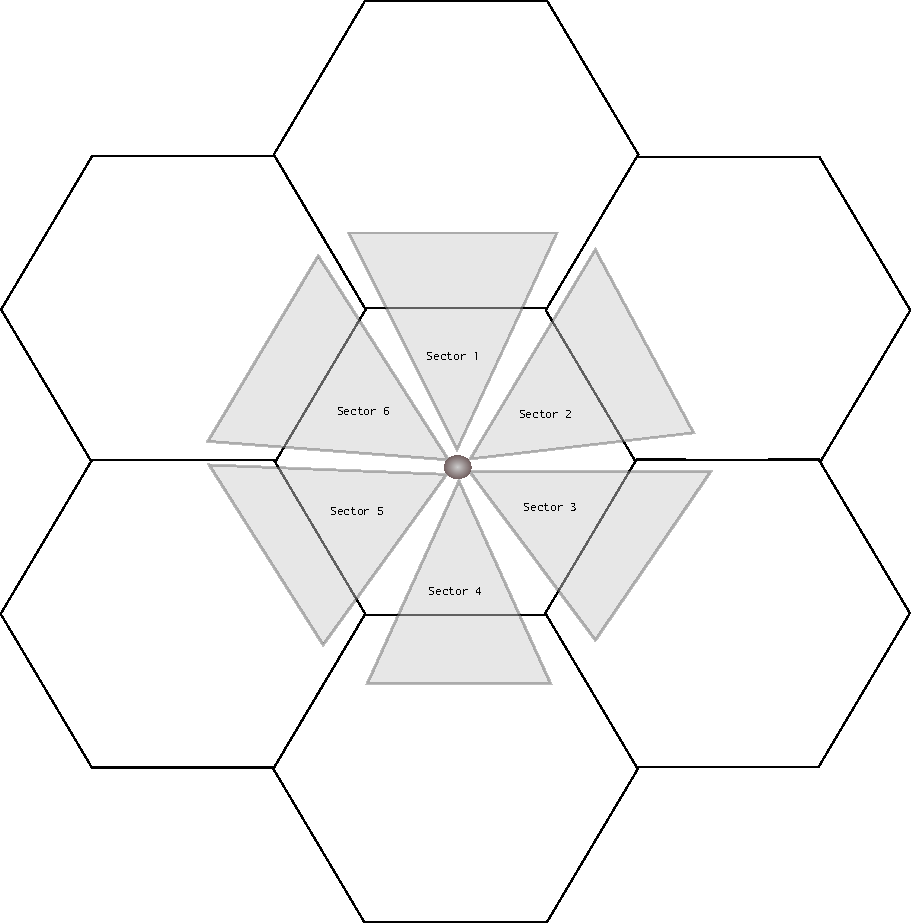
\includegraphics[scale=0.5]{tikz-pics/cellsector.pdf}%
\lthtmlpictureZ
\lthtmlcheckvsize\clearpage}

{\newpage\clearpage
\lthtmlinlinemathA{tex2html_wrap_inline14896}%
$ \frac{360\,^{\circ}}{n}$%
\lthtmlinlinemathZ
\lthtmlcheckvsize\clearpage}

{\newpage\clearpage
\lthtmlinlinemathA{tex2html_wrap_inline14898}%
$ {n}$%
\lthtmlinlinemathZ
\lthtmlcheckvsize\clearpage}

{\newpage\clearpage
\lthtmlinlinemathA{tex2html_wrap_inline14900}%
$ 120^\circ$%
\lthtmlinlinemathZ
\lthtmlcheckvsize\clearpage}

\stepcounter{subsection}
\stepcounter{subsection}
\stepcounter{paragraph}
\stepcounter{paragraph}
\stepcounter{paragraph}
\stepcounter{subsection}
\stepcounter{paragraph}
\stepcounter{paragraph}
\stepcounter{section}
\stepcounter{section}
{\newpage\clearpage
\lthtmlinlinemathA{tex2html_wrap_inline14912}%
$ W$%
\lthtmlinlinemathZ
\lthtmlcheckvsize\clearpage}

{\newpage\clearpage
\lthtmlinlinemathA{tex2html_wrap_inline14916}%
$ W/N$%
\lthtmlinlinemathZ
\lthtmlcheckvsize\clearpage}

{\newpage\clearpage
\lthtmlfigureA{figure974}%
\begin{figure}	\begin{centering}
		%
\begin{tikzpicture}[]
	\begin{scope}[node distance=0cm]
		\node (startSquare) at (-6.0,0.5) [shape=rectangle,draw=black,minimum height = 0.75cm,minimum width = 0.8cm]{   };
		\node (secondSquare) [right = of startSquare,shape=rectangle,draw=black,minimum height = 0.75cm,minimum width = 0.8cm]{   };
		\node (TS0) [right = of secondSquare, shape=rectangle,draw=black,fill=gray!40,minimum height = 0.75cm,minimum width = 0.8cm]{TS1};
		\node (TS1) [right = of TS0, shape=rectangle,draw=black,fill=gray!40,minimum height = 0.75cm,minimum width = 0.8cm]{TS2};
		\node (TS2) [right = of TS1, shape=rectangle,draw=black,fill=gray!40,minimum height = 0.75cm,minimum width = 0.8cm]{TS3};
		\node (TS3) [right = of TS2, shape=rectangle,draw=black,fill=gray!40,minimum height = 0.75cm,minimum width = 0.8cm]{TS4};
		\node (TS4) [right = of TS3, shape=rectangle,draw=black,fill=gray!40,minimum height = 0.75cm,minimum width = 0.8cm]{TS5};
		\node (TS5) [right = of TS4, shape=rectangle,draw=black,fill=gray!40,minimum height = 0.75cm,minimum width = 0.8cm]{TS6};
		\node (TS6) [right = of TS5, shape=rectangle,draw=black,fill=gray!40,minimum height = 0.75cm,minimum width = 0.8cm]{TS7};
		\node (TS7) [right = of TS6, shape=rectangle,draw=black,fill=gray!40,minimum height = 0.75cm,minimum width = 0.8cm]{TS8};
		\node (secondLastSquare) [right = of TS7, shape=rectangle,draw=black,minimum height = 0.75cm,minimum width = 0.8cm]{   };
		\node (lastSquare) [right = of secondLastSquare, shape=rectangle,draw=black,minimum height = 0.75cm,minimum width = 0.8cm]{   };
	\end{scope}
	\node (startF) at (startSquare.west) [above=1.5cm]{};
	\node (endF) at (lastSquare.east) [above=1.5cm]{};
	\draw [|<->|,thick] (startF) to node [above=0.05cm] {Frequency} (endF);
	\draw[decorate,decoration={brace,amplitude = 0.5cm,raise=0.5cm}] (TS0.west) to node [above=1cm] {TDMA Frame} (TS7.east);
	\node (logicalChannel) [shape=rectangle,draw=black,below = 1.5cm of TS4] {Logical Channel};
	\draw (logicalChannel.north east) to (TS1.south east);
	\draw (logicalChannel.north west) to (TS1.south west);
\end{tikzpicture}
		
	\end{centering}
\end{figure}%
\lthtmlfigureZ
\lthtmlcheckvsize\clearpage}

\stepcounter{section}
\stepcounter{section}
\stepcounter{chapter}
\stepcounter{section}
\stepcounter{section}
{\newpage\clearpage
\lthtmlinlinemathA{tex2html_wrap_inline14932}%
$ O(n)$%
\lthtmlinlinemathZ
\lthtmlcheckvsize\clearpage}

{\newpage\clearpage
\lthtmlinlinemathA{tex2html_wrap_inline14934}%
$ O(n^k)$%
\lthtmlinlinemathZ
\lthtmlcheckvsize\clearpage}

{\newpage\clearpage
\lthtmlinlinemathA{tex2html_wrap_inline14936}%
$ k$%
\lthtmlinlinemathZ
\lthtmlcheckvsize\clearpage}

{\newpage\clearpage
\lthtmlinlinemathA{tex2html_wrap_inline14938}%
$ n$%
\lthtmlinlinemathZ
\lthtmlcheckvsize\clearpage}

{\newpage\clearpage
\lthtmlinlinemathA{tex2html_wrap_inline14940}%
$ O(n),O(\log n)$%
\lthtmlinlinemathZ
\lthtmlcheckvsize\clearpage}

{\newpage\clearpage
\lthtmlinlinemathA{tex2html_wrap_inline14942}%
$ O(n^2)$%
\lthtmlinlinemathZ
\lthtmlcheckvsize\clearpage}

\stepcounter{section}
\stepcounter{section}
\stepcounter{subsection}
\stepcounter{subsection}
\stepcounter{section}
{\newpage\clearpage
\lthtmlfigureA{figure1623}%
\begin{figure}	\begin{centering}
	%
\begin{tikzpicture}[]
	%\draw[step=.5cm,gray,very thin] (-0.5,-0.5) grid(10,5);
	\draw[->](-0.5,0) to node[below=0.25cm]{\tiny {f (Mhz)}} (10,0);
	\draw[->](0,-0.5) to node[left=0.25cm] {\tiny {Power (dB)}} (0,5);
	\draw[pattern=vertical lines,thick] (0,0) parabola bend(3,4) (6,0);
	\draw[pattern=horizontal lines,thick] (0,0) parabola bend(3,2) (6,0);
	\draw[-] (0,2) -- (7,2);
	\draw[-] (0,4) -- (7,4);
	\draw[<->,thick] (6.5,2) to node[right=0.25cm]{\tiny {Wanted frequency}} (6.5,4);
	\draw[->,thick] (6.5,0) to node[right=0.25cm]{\tiny {Interfering Frequency}} (6.5,2);
\end{tikzpicture}
	
	\end{centering}
\end{figure}%
\lthtmlfigureZ
\lthtmlcheckvsize\clearpage}

{\newpage\clearpage
\lthtmlfigureA{figure1732}%
\begin{figure}	\begin{centering}
	%
\begin{tikzpicture}[]
	%\draw[step=.5cm,gray,very thin] (-0.5,-0.5) grid(10,5);
	\draw(-0.5,0) -- (10,0);
	\draw(0,-0.5) -- (0,5);
	\draw[pattern=crosshatch dots,even odd rule] (0,0) parabola bend(2.5,4) (5,0) (4.5,0) parabola bend(7,4) (10,0);
	\draw[-] (2.5,0) -- (2.5,4.5);
	\node (interference) at (4.75,3.25) {\tiny {Interference}};
	\draw[<-] (4.75,0.25) -- (interference);
	\draw[-] (7,0) -- (7,4.5);
	\draw[<->] (2.5,4.25) -- (7,4.25);
\end{tikzpicture}
	
	\end{centering}
\end{figure}%
\lthtmlfigureZ
\lthtmlcheckvsize\clearpage}

{\newpage\clearpage
\lthtmlinlinemathA{tex2html_wrap_inline14955}%
$ f_a,f_b,f_c,f_d$%
\lthtmlinlinemathZ
\lthtmlcheckvsize\clearpage}

{\newpage\clearpage
\lthtmlinlinemathA{tex2html_wrap_inline14957}%
$ f_a$%
\lthtmlinlinemathZ
\lthtmlcheckvsize\clearpage}

{\newpage\clearpage
\lthtmlfigureA{figure1761}%
\begin{figure}	\begin{centering}
	%
\begin{tikzpicture}[node distance=0cm]
	\foreach \x in {0,1.5,3,4.5}
	{
		\node [regular polygon,regular polygon sides=6,minimum size=1cm,draw] at (\x,1){};
	}
	\foreach \x in {0.75,2.25,3.75}
	{
		\node [regular polygon,regular polygon sides=6,minimum size=1cm,draw] at (\x,0.57){};
		\node [regular polygon,regular polygon sides=6,minimum size=1cm,draw] at (\x,1.43){};
	}
	\node [regular polygon,regular polygon sides=6,minimum size=1cm,draw,fill=gray!40] at (1.5,1.87){\tiny {$f_b$}};
	\node [regular polygon,regular polygon sides=6,minimum size=1cm,draw,fill=gray!40] at (3,1.87){\tiny {$f_d$}};
	\node [regular polygon,regular polygon sides=6,minimum size=1cm,draw] at (4.5,1.87){};
	\node (cella) [regular polygon,regular polygon sides=6,minimum size=1cm,draw] at (0.75,2.29){\tiny {$f_a$}};
	\node (cellb) [regular polygon,regular polygon sides=6,minimum size=1cm,draw,fill=gray!40] at (2.25,2.29){\tiny {$f_c$}};
	\node (cellc) [regular polygon,regular polygon sides=6,minimum size=1cm,draw] at (3.75,2.29){\tiny {$f_a$}};
	\node (fa) at (cella) [above=1cm]{};
	\node (fc) at (cellc) [above=1cm]{};
	\draw[<->,thick] (fa) to node [above=0.15cm] {\tiny {3 cells}} (fc) ;
	\draw[dashed] (cella.center) -- (fa.north);
	\draw[dashed] (cellc.center) -- (fc.north);
\end{tikzpicture}
	
	\end{centering}
\end{figure}%
\lthtmlfigureZ
\lthtmlcheckvsize\clearpage}

{\newpage\clearpage
\lthtmlinlinemathA{tex2html_wrap_indisplay14961}%
$\displaystyle s  	SINR$%
\lthtmlindisplaymathZ
\lthtmlcheckvsize\clearpage}

{\newpage\clearpage
\lthtmlinlinemathA{tex2html_wrap_indisplay14962}%
$\displaystyle = \frac{P_r}{N_0 + P_I}$%
\lthtmlindisplaymathZ
\lthtmlcheckvsize\clearpage}

{\newpage\clearpage
\lthtmlinlinemathA{tex2html_wrap_indisplay14963}%
$\displaystyle SIR$%
\lthtmlindisplaymathZ
\lthtmlcheckvsize\clearpage}

{\newpage\clearpage
\lthtmlinlinemathA{tex2html_wrap_indisplay14964}%
$\displaystyle = \frac{P_r}{P_I}$%
\lthtmlindisplaymathZ
\lthtmlcheckvsize\clearpage}

{\newpage\clearpage
\lthtmlinlinemathA{tex2html_wrap_inline14966}%
$ P_r$%
\lthtmlinlinemathZ
\lthtmlcheckvsize\clearpage}

{\newpage\clearpage
\lthtmlinlinemathA{tex2html_wrap_inline14968}%
$ P_I$%
\lthtmlinlinemathZ
\lthtmlcheckvsize\clearpage}

{\newpage\clearpage
\lthtmlinlinemathA{tex2html_wrap_inline14970}%
$ N_0$%
\lthtmlinlinemathZ
\lthtmlcheckvsize\clearpage}

\stepcounter{section}
\stepcounter{subsection}
\stepcounter{subsection}
\stepcounter{subsection}
\stepcounter{section}
{\newpage\clearpage
\lthtmlinlinemathA{tex2html_wrap_indisplay14981}%
$\displaystyle G$%
\lthtmlindisplaymathZ
\lthtmlcheckvsize\clearpage}

{\newpage\clearpage
\lthtmlinlinemathA{tex2html_wrap_indisplay14982}%
$\displaystyle = (V,E)$%
\lthtmlindisplaymathZ
\lthtmlcheckvsize\clearpage}

{\newpage\clearpage
\lthtmlinlinemathA{tex2html_wrap_indisplay14983}%
$\displaystyle V$%
\lthtmlindisplaymathZ
\lthtmlcheckvsize\clearpage}

{\newpage\clearpage
\lthtmlinlinemathA{tex2html_wrap_indisplay14984}%
$\displaystyle = \{v_{0},v_{1},\ldots,v_{i}\} | i \in \mathbb{N}$%
\lthtmlindisplaymathZ
\lthtmlcheckvsize\clearpage}

{\newpage\clearpage
\lthtmlinlinemathA{tex2html_wrap_indisplay14985}%
$\displaystyle E$%
\lthtmlindisplaymathZ
\lthtmlcheckvsize\clearpage}

{\newpage\clearpage
\lthtmlinlinemathA{tex2html_wrap_indisplay14986}%
$\displaystyle = \{\{v_0,v_1\},\{v_0,v_2\},\ldots,\{v_i,v_j\}\}|v \in V,\forall ij \in \mathbb{N},i \neq j$%
\lthtmlindisplaymathZ
\lthtmlcheckvsize\clearpage}

{\newpage\clearpage
\lthtmlinlinemathA{tex2html_wrap_indisplay14987}%
$\displaystyle D$%
\lthtmlindisplaymathZ
\lthtmlcheckvsize\clearpage}

{\newpage\clearpage
\lthtmlinlinemathA{tex2html_wrap_indisplay14988}%
$\displaystyle = \{d_{01},d_{02},\ldots,d_{ij}\}| \forall\{i,j\} \in E, \exists d_{ij} \in \mathbb{N}^+$%
\lthtmlindisplaymathZ
\lthtmlcheckvsize\clearpage}

{\newpage\clearpage
\lthtmlinlinemathA{tex2html_wrap_indisplay14989}%
$\displaystyle P$%
\lthtmlindisplaymathZ
\lthtmlcheckvsize\clearpage}

{\newpage\clearpage
\lthtmlinlinemathA{tex2html_wrap_indisplay14990}%
$\displaystyle = \{\{\bar{p_{00}},\overset{=}{p_{01}}\},\{\bar{p_{10}},\overset{=}{p_{11}}\},\ldots,\bar{p_{i0}},\overset{=}{p_{i1}}\}\}| \forall \{i,j\} \in E,\exists p_{ij} \in \mathbb{N}^+$%
\lthtmlindisplaymathZ
\lthtmlcheckvsize\clearpage}

{\newpage\clearpage
\lthtmlinlinemathA{tex2html_wrap_indisplay14991}%
$\displaystyle F$%
\lthtmlindisplaymathZ
\lthtmlcheckvsize\clearpage}

{\newpage\clearpage
\lthtmlinlinemathA{tex2html_wrap_indisplay14992}%
$\displaystyle = \{0,1,2,3,\ldots,k\}| \forall k \in \mathbb{N},\forall v \in V \exists f \in F$%
\lthtmlindisplaymathZ
\lthtmlcheckvsize\clearpage}

{\newpage\clearpage
\lthtmlinlinemathA{tex2html_wrap_indisplay14993}%
$\displaystyle d_{ij}$%
\lthtmlindisplaymathZ
\lthtmlcheckvsize\clearpage}

{\newpage\clearpage
\lthtmlinlinemathA{tex2html_wrap_indisplay14994}%
$\displaystyle < |f(i) - f(j)|, \forall ij \in \mathbb{N},i \neq j$%
\lthtmlindisplaymathZ
\lthtmlcheckvsize\clearpage}

{\newpage\clearpage
\lthtmlinlinemathA{tex2html_wrap_inline14996}%
$ G$%
\lthtmlinlinemathZ
\lthtmlcheckvsize\clearpage}

{\newpage\clearpage
\lthtmlinlinemathA{tex2html_wrap_inline14998}%
$ V$%
\lthtmlinlinemathZ
\lthtmlcheckvsize\clearpage}

{\newpage\clearpage
\lthtmlinlinemathA{tex2html_wrap_inline15000}%
$ v \in V(G)$%
\lthtmlinlinemathZ
\lthtmlcheckvsize\clearpage}

{\newpage\clearpage
\lthtmlinlinemathA{tex2html_wrap_inline15002}%
$ E$%
\lthtmlinlinemathZ
\lthtmlcheckvsize\clearpage}

{\newpage\clearpage
\lthtmlinlinemathA{tex2html_wrap_inline15004}%
$ v_i$%
\lthtmlinlinemathZ
\lthtmlcheckvsize\clearpage}

{\newpage\clearpage
\lthtmlinlinemathA{tex2html_wrap_inline15006}%
$ v_j$%
\lthtmlinlinemathZ
\lthtmlcheckvsize\clearpage}

{\newpage\clearpage
\lthtmlinlinemathA{tex2html_wrap_inline15008}%
$ d_{ij}$%
\lthtmlinlinemathZ
\lthtmlcheckvsize\clearpage}

{\newpage\clearpage
\lthtmlinlinemathA{tex2html_wrap_inline15010}%
$ p_{ij}$%
\lthtmlinlinemathZ
\lthtmlcheckvsize\clearpage}

{\newpage\clearpage
\lthtmlinlinemathA{tex2html_wrap_inline15020}%
$ f(i)$%
\lthtmlinlinemathZ
\lthtmlcheckvsize\clearpage}

{\newpage\clearpage
\lthtmlinlinemathA{tex2html_wrap_inline15030}%
$ P$%
\lthtmlinlinemathZ
\lthtmlcheckvsize\clearpage}

{\newpage\clearpage
\lthtmlinlinemathA{tex2html_wrap_inline15034}%
$ \bar{p_{i0}}$%
\lthtmlinlinemathZ
\lthtmlcheckvsize\clearpage}

{\newpage\clearpage
\lthtmlinlinemathA{tex2html_wrap_inline15036}%
$ \overset{=}{p_{i1}}$%
\lthtmlinlinemathZ
\lthtmlcheckvsize\clearpage}

{\newpage\clearpage
\lthtmlinlinemathA{tex2html_wrap_inline15042}%
$ = (V,E,D,P,F)$%
\lthtmlinlinemathZ
\lthtmlcheckvsize\clearpage}

{\newpage\clearpage
\lthtmlinlinemathA{tex2html_wrap_inline15044}%
$ f: V \rightarrow F$%
\lthtmlinlinemathZ
\lthtmlcheckvsize\clearpage}

{\newpage\clearpage
\lthtmlinlinemathA{tex2html_wrap_inline15046}%
$ c(p_i)$%
\lthtmlinlinemathZ
\lthtmlcheckvsize\clearpage}

{\newpage\clearpage
\lthtmlinlinemathA{tex2html_wrap_indisplay15051}%
$\displaystyle c(p_i)$%
\lthtmlindisplaymathZ
\lthtmlcheckvsize\clearpage}

{\newpage\clearpage
\lthtmlinlinemathA{tex2html_wrap_indisplay15052}%
$\displaystyle =   \begin{cases} 	\bar{p_{i0}} &,$%
\lthtmlindisplaymathZ
\lthtmlcheckvsize\clearpage}

{\newpage\clearpage
\lthtmlinlinemathA{tex2html_wrap_inline15054}%
$ |f(i) - f(j)| = 0$%
\lthtmlinlinemathZ
\lthtmlcheckvsize\clearpage}

{\newpage\clearpage
\lthtmlinlinemathA{tex2html_wrap_indisplay15055}%
$\displaystyle \\\overset{=}{p_{i1}} &,$%
\lthtmlindisplaymathZ
\lthtmlcheckvsize\clearpage}

{\newpage\clearpage
\lthtmlinlinemathA{tex2html_wrap_inline15057}%
$ |f(i) - f(j)| \leqslant d_{ij}$%
\lthtmlinlinemathZ
\lthtmlcheckvsize\clearpage}

{\newpage\clearpage
\lthtmlinlinemathA{tex2html_wrap_indisplay15058}%
$\displaystyle \\0 &,$%
\lthtmlindisplaymathZ
\lthtmlcheckvsize\clearpage}

{\newpage\clearpage
\lthtmlinlinemathA{tex2html_wrap_inline15060}%
$ |f(i) - f(j)| > d_{ij}$%
\lthtmlinlinemathZ
\lthtmlcheckvsize\clearpage}

{\newpage\clearpage
\lthtmlinlinemathA{tex2html_wrap_indisplay15061}%
$\displaystyle \end{cases}$%
\lthtmlindisplaymathZ
\lthtmlcheckvsize\clearpage}

{\newpage\clearpage
\lthtmlinlinemathA{tex2html_wrap_indisplay15062}%
$\displaystyle Total Interference$%
\lthtmlindisplaymathZ
\lthtmlcheckvsize\clearpage}

{\newpage\clearpage
\lthtmlinlinemathA{tex2html_wrap_indisplay15063}%
$\displaystyle = \sum^{|P|}_{i = 0}c(p_i),p \in P$%
\lthtmlindisplaymathZ
\lthtmlcheckvsize\clearpage}

\stepcounter{section}
\stepcounter{subsection}
{\newpage\clearpage
\lthtmlinlinemathA{tex2html_wrap_inline15067}%
$ d$%
\lthtmlinlinemathZ
\lthtmlcheckvsize\clearpage}

\stepcounter{subsection}
\stepcounter{subsection}
\stepcounter{subsubsection}
{\newpage\clearpage
\lthtmlinlinemathA{tex2html_wrap_inline15072}%
$ F = \{16,17,18,\dots,90\}$%
\lthtmlinlinemathZ
\lthtmlcheckvsize\clearpage}

{\newpage\clearpage
\lthtmlinlinemathA{tex2html_wrap_inline15074}%
$ F= \{36,37,38,\dots,67\}$%
\lthtmlinlinemathZ
\lthtmlcheckvsize\clearpage}

{\newpage\clearpage
\lthtmlinlinemathA{tex2html_wrap_inline15076}%
$ F= \{16,17,\dots,35\}$%
\lthtmlinlinemathZ
\lthtmlcheckvsize\clearpage}

{\newpage\clearpage
\lthtmlinlinemathA{tex2html_wrap_inline15078}%
$ F= \{68,69,70,\dots,90\}$%
\lthtmlinlinemathZ
\lthtmlcheckvsize\clearpage}

\stepcounter{subsubsection}
{\newpage\clearpage
\lthtmlinlinemathA{tex2html_wrap_inline15081}%
$ F = \{42,43,44,45,46\}$%
\lthtmlinlinemathZ
\lthtmlcheckvsize\clearpage}

{\newpage\clearpage
\lthtmlinlinemathA{tex2html_wrap_inline15083}%
$ F= \{53,54,55,\dots,124\}$%
\lthtmlinlinemathZ
\lthtmlcheckvsize\clearpage}

{\newpage\clearpage
\lthtmlinlinemathA{tex2html_wrap_inline15085}%
$ F = \{47,48,49,50,51,52\}$%
\lthtmlinlinemathZ
\lthtmlcheckvsize\clearpage}

\stepcounter{subsubsection}
{\newpage\clearpage
\lthtmlinlinemathA{tex2html_wrap_inline15088}%
$ F= \{681,682,683, \dots, 735\}$%
\lthtmlinlinemathZ
\lthtmlcheckvsize\clearpage}

\stepcounter{subsubsection}
{\newpage\clearpage
\lthtmlinlinemathA{tex2html_wrap_inline15091}%
$ F = \{56,57,58,\dots,94\}$%
\lthtmlinlinemathZ
\lthtmlcheckvsize\clearpage}

\stepcounter{section}
\stepcounter{subsection}
\stepcounter{subsection}
\stepcounter{subsection}
\stepcounter{subsection}
\stepcounter{subsection}
\stepcounter{section}
\stepcounter{chapter}
\stepcounter{section}
\stepcounter{section}
\stepcounter{section}
\stepcounter{section}
\stepcounter{subsection}
\stepcounter{subsection}
\stepcounter{subsubsection}
\stepcounter{subsubsection}
\stepcounter{subsubsection}
\stepcounter{subsubsection}
\stepcounter{subsection}
{\newpage\clearpage
\lthtmlfigureA{algorithm2593}%
\begin{algorithm}
% latex2html id marker 2593
[H]
\caption{Basic Tabu Search Algorithm\cite{TabuRCAProblem,TabuMontemanniSmith}}
	\begin{algorithmic}[1]
		\State Initialize parameters
    \State $\hat{x_0} \leftarrow$\  Initialize starting solution
		\While{stopping criteria not met}
    \State $\hat{y_i} \leftarrow$\  Determine $\hat{x_i}$\  neighbourhood solutions 
    \State Evaluate neighbouring solutions with fitness function $f(\hat{y_i})$
    \State $\hat{z_i} \leftarrow$Select best neighbour from $\hat{y_i}$
    \If{Move to $\hat{z_i}$\  is Tabu}
    \If{$\hat{z_i}$\  meets Aspiration Criterion}
    \State $\hat{x_i} \leftarrow \hat{z_i}$
				\EndIf
			\Else
      \State Add $\hat{x_i}$\  to Tabu List
      \State $\hat{x_i} \leftarrow \hat{z_i}$
      \If{$\hat{x_i}$\  repeated $\ge$\  max repeats}
					\State diversify()
				\Else
					\State intensify()
				\EndIf
			\EndIf
		\EndWhile
    \State Return $\hat{x_i}$\  as best found solution
	\end{algorithmic}
\end{algorithm}%
\lthtmlfigureZ
\lthtmlcheckvsize\clearpage}

{\newpage\clearpage
\lthtmlinlinemathA{tex2html_wrap_inline15116}%
$ x_i$%
\lthtmlinlinemathZ
\lthtmlcheckvsize\clearpage}

{\newpage\clearpage
\lthtmlinlinemathA{tex2html_wrap_inline15118}%
$ y_i$%
\lthtmlinlinemathZ
\lthtmlcheckvsize\clearpage}

{\newpage\clearpage
\lthtmlinlinemathA{tex2html_wrap_inline15120}%
$ f(y_i)$%
\lthtmlinlinemathZ
\lthtmlcheckvsize\clearpage}

{\newpage\clearpage
\lthtmlinlinemathA{tex2html_wrap_inline15122}%
$ z_i$%
\lthtmlinlinemathZ
\lthtmlcheckvsize\clearpage}

\stepcounter{subsection}
\stepcounter{paragraph}
\stepcounter{paragraph}
\stepcounter{paragraph}
\stepcounter{section}
\stepcounter{subsection}
{\newpage\clearpage
\lthtmlinlinemathA{tex2html_wrap_indisplay15168}%
$\displaystyle M_{AC} = 	\begin{cases} 	1, &\text{if $f(y) \leq f(x)$}\\e^{-\frac{\Delta E}{T_k}} , &\text{otherwise}\\\end{cases}$%
\lthtmlindisplaymathZ
\lthtmlcheckvsize\clearpage}

{\newpage\clearpage
\lthtmlinlinemathA{tex2html_wrap_inline15170}%
$ f$%
\lthtmlinlinemathZ
\lthtmlcheckvsize\clearpage}

{\newpage\clearpage
\lthtmlinlinemathA{tex2html_wrap_inline15172}%
$ T_k$%
\lthtmlinlinemathZ
\lthtmlcheckvsize\clearpage}

{\newpage\clearpage
\lthtmlinlinemathA{tex2html_wrap_inline15176}%
$ \Delta E$%
\lthtmlinlinemathZ
\lthtmlcheckvsize\clearpage}

{\newpage\clearpage
\lthtmlinlinemathA{tex2html_wrap_inline15178}%
$ x$%
\lthtmlinlinemathZ
\lthtmlcheckvsize\clearpage}

{\newpage\clearpage
\lthtmlinlinemathA{tex2html_wrap_inline15180}%
$ y$%
\lthtmlinlinemathZ
\lthtmlcheckvsize\clearpage}

\stepcounter{subsection}
\stepcounter{subsubsection}
{\newpage\clearpage
\lthtmlinlinemathA{tex2html_wrap_indisplay15184}%
$\displaystyle T_k = \frac{T_0}{ln(k)},$%
\lthtmlindisplaymathZ
\lthtmlcheckvsize\clearpage}

{\newpage\clearpage
\lthtmlinlinemathA{tex2html_wrap_indisplay15185}%
$\displaystyle k \neq 0\\$%
\lthtmlindisplaymathZ
\lthtmlcheckvsize\clearpage}

{\newpage\clearpage
\lthtmlinlinemathA{tex2html_wrap_indisplay15191}%
$\displaystyle T_k = \frac{T_0}{k} ~, k \neq 0$%
\lthtmlindisplaymathZ
\lthtmlcheckvsize\clearpage}

{\newpage\clearpage
\lthtmlinlinemathA{tex2html_wrap_indisplay15193}%
$\displaystyle T(k)=T_0e^{-C_k},$%
\lthtmlindisplaymathZ
\lthtmlcheckvsize\clearpage}

\stepcounter{subsubsection}
\stepcounter{subsubsection}
\stepcounter{subsubsection}
\stepcounter{subsection}
{\newpage\clearpage
\lthtmlfigureA{algorithm2787}%
\begin{algorithm}
% latex2html id marker 2787
[H]
\caption{Basic Simulated Annealing Algorithm\cite{VeryFastSAImageEnchancement,ChaosSA}}
	\begin{algorithmic}[1]
		\State Initialize parameters
		\State Set starting temperature $T(0)$
    \State $\hat{x_0} \leftarrow$\  Generate initial starting solution
		\While{Stopping criterion not met}
    \State $\hat{y_i} \leftarrow$\  Generate neighbouring solutions to $\hat{x_i}$
    \State Evaluate $\hat{y_i}$\  neighbours with fitness function $f(\hat{y_i})$
    \State Calculate probability $\hat{p_i}$\  of $\hat{y_i}$\  neighbours with equation~\ref{eq:saprobability}
    \State $\hat{x_i} \leftarrow$\  Select $\hat{y_i}$\  neighbour based on probability $p_i$
			\State Reduce temperature $T(i)$\  based on cooling schedule
		\EndWhile
    \State Return best solution $\hat{x_i}$
	\end{algorithmic}
\end{algorithm}%
\lthtmlfigureZ
\lthtmlcheckvsize\clearpage}

\stepcounter{subsection}
\stepcounter{paragraph}
\stepcounter{paragraph}
\stepcounter{paragraph}
\stepcounter{section}
\stepcounter{subsection}
\stepcounter{subsection}
\stepcounter{subsubsection}
\stepcounter{subsubsection}
\stepcounter{subsubsection}
\stepcounter{subsubsection}
\stepcounter{subsubsection}
\stepcounter{subsection}
{\newpage\clearpage
\lthtmlfigureA{algorithm3004}%
\begin{algorithm}
% latex2html id marker 3004
[H]
\caption{Basic Genetic Algorithm Algorithm\cite{FamilyGA,AdaptiveSAGA,DistributedHierarchicalGA,SelfAdaptiveGA}}
	\begin{algorithmic}[1]
		\State $pop_n\leftarrow$Initialize population
		\While{Stopping criteria is not met}
    \State Evaluate individuals of population with fitness function $f(\hat{x_i})$
    \State $\hat{y_k} \leftarrow$\  Select parent individuals from population using selection operator
		\Repeat
    \For{Each chromosome $\hat{g_i}$\  in $\hat{y_{k-1}}$}
    \State $\hat{c_i} \leftarrow$\  calculate crossover porbability for $\hat{g_i}$
    \If{$\hat{c_i} \geq$\  Crossover threshold}
    \State $\hat{g_i} \leftarrow$\  Apply crossover operator to $\hat{g_i}$
				\EndIf
        \State $\hat{o_i} \leftarrow \hat{g_i}$
        \State $\hat{m_i}\leftarrow$\  Calculate Mutation probability for $\hat{o_i}$
        \If{$\hat{m_i} \geq$\  Mutation threshold}
        \State Apply mutation operator to $\hat{o_i}$
				\EndIf
        \State Add offspring chromosome $\hat{o_i}$\  to $new_{pop}$
			\EndFor
		\Until{$size(new_{pop}) = size(pop_n)$}
		\State $pop_n \leftarrow$\  select new population from $pop_n$\  and $new_{pop}$
		\EndWhile
    \State $\hat{x_i} \leftarrow$\  Determine best chromosome in $pop_n$
    \State Return best solution $\hat{x_i}$
	\end{algorithmic}
\end{algorithm}%
\lthtmlfigureZ
\lthtmlcheckvsize\clearpage}

{\newpage\clearpage
\lthtmlinlinemathA{tex2html_wrap_inline15239}%
$ pop_n$%
\lthtmlinlinemathZ
\lthtmlcheckvsize\clearpage}

{\newpage\clearpage
\lthtmlinlinemathA{tex2html_wrap_inline15241}%
$ n > 0$%
\lthtmlinlinemathZ
\lthtmlcheckvsize\clearpage}

{\newpage\clearpage
\lthtmlinlinemathA{tex2html_wrap_inline15243}%
$ f(\hat{x_i})$%
\lthtmlinlinemathZ
\lthtmlcheckvsize\clearpage}

{\newpage\clearpage
\lthtmlinlinemathA{tex2html_wrap_inline15245}%
$ \hat{g_i}$%
\lthtmlinlinemathZ
\lthtmlcheckvsize\clearpage}

{\newpage\clearpage
\lthtmlinlinemathA{tex2html_wrap_inline15249}%
$ \hat{o_i}$%
\lthtmlinlinemathZ
\lthtmlcheckvsize\clearpage}

\stepcounter{subsection}
\stepcounter{paragraph}
\stepcounter{paragraph}
\stepcounter{paragraph}
\stepcounter{section}
\stepcounter{chapter}
\stepcounter{section}
\stepcounter{section}
\stepcounter{section}
\stepcounter{subsection}


\setlength%

\setlength{}{}


\setlength%

\setlength{}{}
{\newpage\clearpage
\lthtmlinlinemathA{tex2html_wrap_inline5110}%
\fbox{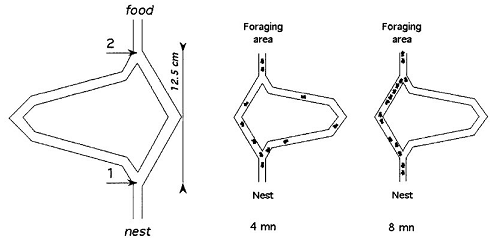
\includegraphics[width=4.0in,height=2.0in]{./pictures/antBridgeExperiment.png}}%
\lthtmlinlinemathZ
\lthtmlcheckvsize\clearpage}

\stepcounter{subsection}
\stepcounter{subsubsection}
\stepcounter{subsubsection}
{\newpage\clearpage
\lthtmlinlinemathA{tex2html_wrap_indisplay15317}%
$\displaystyle \tau_{ij}(t) = (1-p)\tau_{ij}(t), p\in [0,1]$%
\lthtmlindisplaymathZ
\lthtmlcheckvsize\clearpage}

{\newpage\clearpage
\lthtmlinlinemathA{tex2html_wrap_inline15319}%
$ p$%
\lthtmlinlinemathZ
\lthtmlcheckvsize\clearpage}

{\newpage\clearpage
\lthtmlinlinemathA{tex2html_wrap_inline15321}%
$ p=1$%
\lthtmlinlinemathZ
\lthtmlcheckvsize\clearpage}

\stepcounter{subsubsection}
{\newpage\clearpage
\lthtmlinlinemathA{tex2html_wrap_indisplay15326}%
$\displaystyle p^k_{ij}(t) = \begin{cases} 	\frac{\tau^{\alpha}_{ij}(t)\eta^{\beta}_{ij}}{\sum_{u \in N^k_i(t)} {\tau^{\alpha}_{iu}(t)\eta^{\beta}_{iu}(t)}}, &\text{if $j \in N^k_i(t)$}\\0, &\text{if $j \notin N^k_i(t)$}\\\end{cases}$%
\lthtmlindisplaymathZ
\lthtmlcheckvsize\clearpage}

{\newpage\clearpage
\lthtmlinlinemathA{tex2html_wrap_inline15332}%
$ j$%
\lthtmlinlinemathZ
\lthtmlcheckvsize\clearpage}

{\newpage\clearpage
\lthtmlinlinemathA{tex2html_wrap_inline15334}%
$ \tau_{ij}$%
\lthtmlinlinemathZ
\lthtmlcheckvsize\clearpage}

{\newpage\clearpage
\lthtmlinlinemathA{tex2html_wrap_inline15340}%
$ \eta_{ij}$%
\lthtmlinlinemathZ
\lthtmlcheckvsize\clearpage}

{\newpage\clearpage
\lthtmlinlinemathA{tex2html_wrap_inline15346}%
$ \alpha$%
\lthtmlinlinemathZ
\lthtmlcheckvsize\clearpage}

{\newpage\clearpage
\lthtmlinlinemathA{tex2html_wrap_inline15348}%
$ \beta$%
\lthtmlinlinemathZ
\lthtmlcheckvsize\clearpage}

{\newpage\clearpage
\lthtmlinlinemathA{tex2html_wrap_inline15350}%
$ \alpha=\beta$%
\lthtmlinlinemathZ
\lthtmlcheckvsize\clearpage}

{\newpage\clearpage
\lthtmlinlinemathA{tex2html_wrap_inline15352}%
$ \alpha = 0$%
\lthtmlinlinemathZ
\lthtmlcheckvsize\clearpage}

{\newpage\clearpage
\lthtmlinlinemathA{tex2html_wrap_inline15358}%
$ \beta = 0$%
\lthtmlinlinemathZ
\lthtmlcheckvsize\clearpage}

{\newpage\clearpage
\lthtmlinlinemathA{tex2html_wrap_inline15364}%
$ j \in N^k_i(t)$%
\lthtmlinlinemathZ
\lthtmlcheckvsize\clearpage}

\stepcounter{subsubsection}
{\newpage\clearpage
\lthtmlinlinemathA{tex2html_wrap_indisplay15372}%
$\displaystyle \tau_{ij}(t+1)$%
\lthtmlindisplaymathZ
\lthtmlcheckvsize\clearpage}

{\newpage\clearpage
\lthtmlinlinemathA{tex2html_wrap_indisplay15373}%
$\displaystyle = \tau_{ij}(t) + \Delta\tau_{ij}(t),$%
\lthtmlindisplaymathZ
\lthtmlcheckvsize\clearpage}

{\newpage\clearpage
\lthtmlinlinemathA{tex2html_wrap_indisplay15374}%
$\displaystyle \Delta\tau_{ij}$%
\lthtmlindisplaymathZ
\lthtmlcheckvsize\clearpage}

{\newpage\clearpage
\lthtmlinlinemathA{tex2html_wrap_indisplay15375}%
$\displaystyle = \sum^{n_k}_{k=1}\Delta\tau^k_{ij}(t)$%
\lthtmlindisplaymathZ
\lthtmlcheckvsize\clearpage}

{\newpage\clearpage
\lthtmlinlinemathA{tex2html_wrap_inline15377}%
$ \tau_{ij}(t+1)$%
\lthtmlinlinemathZ
\lthtmlcheckvsize\clearpage}

{\newpage\clearpage
\lthtmlinlinemathA{tex2html_wrap_inline15379}%
$ (t+1)$%
\lthtmlinlinemathZ
\lthtmlcheckvsize\clearpage}

{\newpage\clearpage
\lthtmlinlinemathA{tex2html_wrap_inline15383}%
$ (i,j)$%
\lthtmlinlinemathZ
\lthtmlcheckvsize\clearpage}

{\newpage\clearpage
\lthtmlinlinemathA{tex2html_wrap_inline15385}%
$ \Delta\tau_{ij}$%
\lthtmlinlinemathZ
\lthtmlcheckvsize\clearpage}

{\newpage\clearpage
\lthtmlinlinemathA{tex2html_wrap_indisplay15389}%
$\displaystyle = (1 - p_1)\tau_{ij}(t) + p_1\Delta\tau_{ij}(t),$%
\lthtmlindisplaymathZ
\lthtmlcheckvsize\clearpage}

{\newpage\clearpage
\lthtmlinlinemathA{tex2html_wrap_indisplay15391}%
$\displaystyle =  	\begin{cases} 		\frac{1}{f(x^+(t))} &$%
\lthtmlindisplaymathZ
\lthtmlcheckvsize\clearpage}

{\newpage\clearpage
\lthtmlinlinemathA{tex2html_wrap_inline15393}%
$ (i,j) \in x+(t)$%
\lthtmlinlinemathZ
\lthtmlcheckvsize\clearpage}

{\newpage\clearpage
\lthtmlinlinemathA{tex2html_wrap_indisplay15394}%
$\displaystyle \\0 &$%
\lthtmlindisplaymathZ
\lthtmlcheckvsize\clearpage}

{\newpage\clearpage
\lthtmlinlinemathA{tex2html_wrap_inline15397}%
$ f(x^+(t))$%
\lthtmlinlinemathZ
\lthtmlcheckvsize\clearpage}

{\newpage\clearpage
\lthtmlinlinemathA{tex2html_wrap_inline15399}%
$ p_1$%
\lthtmlinlinemathZ
\lthtmlcheckvsize\clearpage}

{\newpage\clearpage
\lthtmlinlinemathA{tex2html_wrap_inline15401}%
$ \Delta\tau_{ij}(t)$%
\lthtmlinlinemathZ
\lthtmlcheckvsize\clearpage}

{\newpage\clearpage
\lthtmlinlinemathA{tex2html_wrap_inline15403}%
$ t$%
\lthtmlinlinemathZ
\lthtmlcheckvsize\clearpage}

{\newpage\clearpage
\lthtmlinlinemathA{tex2html_wrap_inline15405}%
$ ij$%
\lthtmlinlinemathZ
\lthtmlcheckvsize\clearpage}

{\newpage\clearpage
\lthtmlinlinemathA{tex2html_wrap_indisplay15407}%
$\displaystyle \tau_{ij}(t) = (1 - p_2)\tau_{ij} + p_2\tau_0$%
\lthtmlindisplaymathZ
\lthtmlcheckvsize\clearpage}

{\newpage\clearpage
\lthtmlinlinemathA{tex2html_wrap_inline15409}%
$ \tau_0$%
\lthtmlinlinemathZ
\lthtmlcheckvsize\clearpage}

{\newpage\clearpage
\lthtmlinlinemathA{tex2html_wrap_inline15411}%
$ p_2 \in [0,1]$%
\lthtmlinlinemathZ
\lthtmlcheckvsize\clearpage}

\stepcounter{subsection}
{\newpage\clearpage
\lthtmlfigureA{algorithm4027}%
\begin{algorithm}
% latex2html id marker 4027
[H]
\caption{Ant System Algorithm~\cite{CompuIntelligenceIntro}}
	\begin{algorithmic}[1]
	\State$\text{Initialize $\tau_{ij}$\  with small starting values}$
	\State$t \leftarrow 0$
	\State$\text{Place $n_k$\  ants on starting node}$
	\While{stopping condition not reached}
		\For{each ant $k \leftarrow 0$\  to  number of ants $n_k$}
			\State$p^k(t) \leftarrow \text{Initialize path } p^k \text{for time step } t$
			\Repeat
				\State$\text{Select next node based on probability equation~\ref{eq:ASprobability}}$
				\State$\text{Add link (i,j) to path } p^k(t)$
			\Until{Final node reached}
			\algstore{AS}
	\end{algorithmic}
\addtocounter{algorithm}{-1}
\end{algorithm}%
\lthtmlfigureZ
\lthtmlcheckvsize\clearpage}

{\newpage\clearpage
\lthtmlfigureA{algorithm4045}%
\begin{algorithm}
% latex2html id marker 4045
[H]
\caption{Ant System Algorithm (continued)}
	\begin{algorithmic}
		\algrestore{AS}
			\State$x^k(t) \leftarrow \text{Remove loops from path }p^k(t)$
			\State$\text{Calculate length of path $f(p^k(t)$})$
		\EndFor
		\For{each link $(i,j)$\  in graph}
			\State$\tau_{ij} = \text{Reduce pheromone of link $(i,j)$\  with equation~\ref{eq:pheromoneevapuration}}$
		\EndFor
		\For{each ant $k = 0$\  to  number of ants $n_k$}
			\For{each link $(i,j)$\  in $p^k(t)$}
				\State$\triangle \tau_{ij} = \frac{1}{f(p^k(t))}$
				\State$\text{Update the pheromone $\tau_{ij}$\  with equation~\ref{eq:pheromoneupdate}}$
			\EndFor
		\EndFor
		\State$t \leftarrow t + 1$
	\EndWhile\\
	\Return $\text{path $x^k(t)$\  with the smallest $f(x^k(t))$\  as the solution}$
	\end{algorithmic}
\end{algorithm}%
\lthtmlfigureZ
\lthtmlcheckvsize\clearpage}

\stepcounter{subsection}
\stepcounter{paragraph}
\stepcounter{paragraph}
\stepcounter{section}
\stepcounter{subsection}
\stepcounter{subsection}
\stepcounter{subsubsection}
{\newpage\clearpage
\lthtmlinlinemathA{tex2html_wrap_indisplay15436}%
$\displaystyle p_i = \frac{{fit}_i}{\sum^{SN}_{n=1}{fit}_n}$%
\lthtmlindisplaymathZ
\lthtmlcheckvsize\clearpage}

{\newpage\clearpage
\lthtmlinlinemathA{tex2html_wrap_inline15438}%
$ p_i$%
\lthtmlinlinemathZ
\lthtmlcheckvsize\clearpage}

{\newpage\clearpage
\lthtmlinlinemathA{tex2html_wrap_inline15442}%
$ {fit}_i$%
\lthtmlinlinemathZ
\lthtmlcheckvsize\clearpage}

{\newpage\clearpage
\lthtmlinlinemathA{tex2html_wrap_inline15448}%
$ P_i$%
\lthtmlinlinemathZ
\lthtmlcheckvsize\clearpage}

\stepcounter{subsubsection}
{\newpage\clearpage
\lthtmlinlinemathA{tex2html_wrap_indisplay15453}%
$\displaystyle v_{ij} = x_{ij} + \phi_{ij}(x_{ij} - x_{kj})$%
\lthtmlindisplaymathZ
\lthtmlcheckvsize\clearpage}

{\newpage\clearpage
\lthtmlinlinemathA{tex2html_wrap_inline15455}%
$ k \in \{1,2,\dots,SN\}$%
\lthtmlinlinemathZ
\lthtmlcheckvsize\clearpage}

{\newpage\clearpage
\lthtmlinlinemathA{tex2html_wrap_inline15457}%
$ j \in \{1,2,\dots,D\}$%
\lthtmlinlinemathZ
\lthtmlcheckvsize\clearpage}

{\newpage\clearpage
\lthtmlinlinemathA{tex2html_wrap_inline15467}%
$ x_{ij}$%
\lthtmlinlinemathZ
\lthtmlcheckvsize\clearpage}

{\newpage\clearpage
\lthtmlinlinemathA{tex2html_wrap_inline15469}%
$ \phi_{ij}$%
\lthtmlinlinemathZ
\lthtmlcheckvsize\clearpage}

{\newpage\clearpage
\lthtmlinlinemathA{tex2html_wrap_inline15471}%
$ [-1,1]$%
\lthtmlinlinemathZ
\lthtmlcheckvsize\clearpage}

{\newpage\clearpage
\lthtmlinlinemathA{tex2html_wrap_inline15473}%
$ x_{ij} - x_{kj}$%
\lthtmlinlinemathZ
\lthtmlcheckvsize\clearpage}

\stepcounter{subsubsection}
{\newpage\clearpage
\lthtmlinlinemathA{tex2html_wrap_indisplay15480}%
$\displaystyle x_{ij} = x_{yj} + rand[0,1](x_{zj} - x_{yj})$%
\lthtmlindisplaymathZ
\lthtmlcheckvsize\clearpage}

\stepcounter{subsection}
{\newpage\clearpage
\lthtmlfigureA{algorithm4272}%
\begin{algorithm}
% latex2html id marker 4272
[H]
\caption{Basic Artificial Bee Colony Algorithm\cite{ABCCompareStudy}}
	\begin{algorithmic}[1]
		\State$b_n \leftarrow \text{Initialize bees}$
		\State$s_n \leftarrow \text{Initialize starting solutions}$
		\State$\text{Evaluate starting solutions with fitness function $f(s_n)$}$
		\State$t \leftarrow 0$
		\While{stopping criteria not met}
			\For{each employed bee $eb_i = 0$\  to max bees $b_n$}
				\State$\hat{v_i} \leftarrow \text{Generate new solution with equation~\ref{eq:beeGenerate}}$
				\State$\text{Evaluate with fitness function $f(\hat{v_i})$}$
				\State Apply greedy selection between $\hat{v_i}$\  and the current solution $\hat{s_i}$\  of bee $eb_i$
			\EndFor
			\algstore{ABC}
	\end{algorithmic}
\addtocounter{algorithm}{-1}
\end{algorithm}%
\lthtmlfigureZ
\lthtmlcheckvsize\clearpage}

{\newpage\clearpage
\lthtmlfigureA{algorithm4291}%
\begin{algorithm}
% latex2html id marker 4291

	\caption{Basic Artificial Bee Colony Algorithm (continued)}
	
	\begin{algorithmic}[1]
		\algrestore{ABC}
    \State$\text{Calculate probability $p_i$\  for solutions $\hat{s_i}$\  in $\hat{s_n}$\  using equation~\ref{eq:beeProbability}}$
			\For{each onlooker bee $ob_i \leftarrow 0$\  to max bees $b_n$}
				\State$\hat{x_i} \leftarrow \text{Select solution $\hat{s_i}$\  based on $p_i$} $
				\State$\hat{v_i} \leftarrow \text{Generate new solution with $\hat{x_i}$\  and $p_i$}$
				\State$\text{Evaluate $\hat{v_i}$\  with fitness function $f(\hat{v_i})$}$
				\State$\text{Apply greedy selection between $\hat{v_i}$\  and bee $ob_i$\  current solution}$
			\EndFor
			\If{there is an abandoned solution for a scout bee}
				\State Replace with solution generated with equation~\ref{eq:scoutGenerate}
			\EndIf
			\State$t \leftarrow t + 1$
		\EndWhile
	\end{algorithmic}
\end{algorithm}%
\lthtmlfigureZ
\lthtmlcheckvsize\clearpage}

\stepcounter{subsection}
\stepcounter{paragraph}
\stepcounter{paragraph}
\stepcounter{paragraph}
\stepcounter{section}
\stepcounter{subsection}
\stepcounter{subsection}
\stepcounter{subsubsection}
\stepcounter{subsubsection}
\stepcounter{subsubsection}
{\newpage\clearpage
\lthtmlinlinemathA{tex2html_wrap_indisplay15500}%
$\displaystyle \hat{v}_i(t+1)$%
\lthtmlindisplaymathZ
\lthtmlcheckvsize\clearpage}

{\newpage\clearpage
\lthtmlinlinemathA{tex2html_wrap_indisplay15501}%
$\displaystyle = \hat{v}_i(t) + c_1\hat{\phi}_1(t)[\hat{pbest}_i - \hat{x}_i(t)] + c_2\hat{\phi}_2(t)[\hat{gbest}_i - \hat{x}_i(t)]$%
\lthtmlindisplaymathZ
\lthtmlcheckvsize\clearpage}

{\newpage\clearpage
\lthtmlinlinemathA{tex2html_wrap_indisplay15502}%
$\displaystyle \hat{x}_i(t+1)$%
\lthtmlindisplaymathZ
\lthtmlcheckvsize\clearpage}

{\newpage\clearpage
\lthtmlinlinemathA{tex2html_wrap_indisplay15503}%
$\displaystyle = \hat{x}_i(t) + \hat{v}_i(t+1)$%
\lthtmlindisplaymathZ
\lthtmlcheckvsize\clearpage}

{\newpage\clearpage
\lthtmlinlinemathA{tex2html_wrap_inline15505}%
$ \hat{v}_i(t+1)$%
\lthtmlinlinemathZ
\lthtmlcheckvsize\clearpage}

{\newpage\clearpage
\lthtmlinlinemathA{tex2html_wrap_inline15509}%
$ t+1$%
\lthtmlinlinemathZ
\lthtmlcheckvsize\clearpage}

{\newpage\clearpage
\lthtmlinlinemathA{tex2html_wrap_inline15511}%
$ c_1\hat{\phi}_1(t)[\hat{pbest}_i - \hat{x}_i(t)]$%
\lthtmlinlinemathZ
\lthtmlcheckvsize\clearpage}

{\newpage\clearpage
\lthtmlinlinemathA{tex2html_wrap_inline15513}%
$ c_1$%
\lthtmlinlinemathZ
\lthtmlcheckvsize\clearpage}

{\newpage\clearpage
\lthtmlinlinemathA{tex2html_wrap_inline15515}%
$ c_2\hat{\phi}_2(t)[\hat{gbest}_i - \hat{x}_i(t)]$%
\lthtmlinlinemathZ
\lthtmlcheckvsize\clearpage}

{\newpage\clearpage
\lthtmlinlinemathA{tex2html_wrap_inline15517}%
$ c_2$%
\lthtmlinlinemathZ
\lthtmlcheckvsize\clearpage}

{\newpage\clearpage
\lthtmlinlinemathA{tex2html_wrap_inline15523}%
$ \hat{\phi}_i$%
\lthtmlinlinemathZ
\lthtmlcheckvsize\clearpage}

{\newpage\clearpage
\lthtmlinlinemathA{tex2html_wrap_inline15525}%
$ \hat{\phi}_2$%
\lthtmlinlinemathZ
\lthtmlcheckvsize\clearpage}

{\newpage\clearpage
\lthtmlinlinemathA{tex2html_wrap_inline15527}%
$ [0,1]$%
\lthtmlinlinemathZ
\lthtmlcheckvsize\clearpage}

{\newpage\clearpage
\lthtmlinlinemathA{tex2html_wrap_inline15531}%
$ \hat{x}_i(t)$%
\lthtmlinlinemathZ
\lthtmlcheckvsize\clearpage}

{\newpage\clearpage
\lthtmlinlinemathA{tex2html_wrap_inline5376}%
\fbox{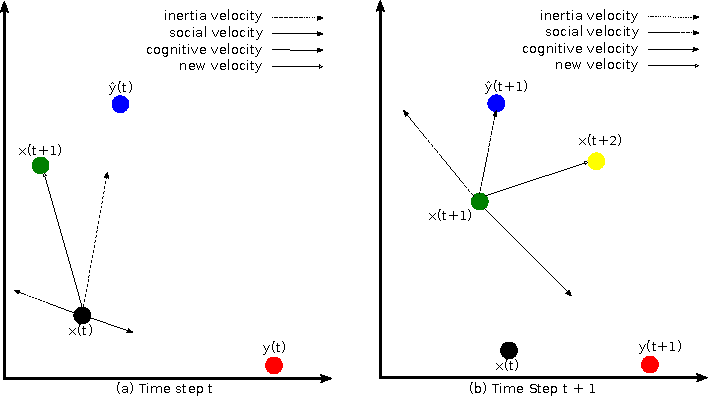
\includegraphics[width=4.5in,height=2.5in]{./pictures/geovelocity.pdf}}%
\lthtmlinlinemathZ
\lthtmlcheckvsize\clearpage}

\stepcounter{subsubsection}
{\newpage\clearpage
\lthtmlinlinemathA{tex2html_wrap_indisplay15539}%
$\displaystyle \hat{v_i}(t+1)$%
\lthtmlindisplaymathZ
\lthtmlcheckvsize\clearpage}

{\newpage\clearpage
\lthtmlinlinemathA{tex2html_wrap_indisplay15540}%
$\displaystyle = 	\begin{cases} 	\hat{v'_i}(t+1), &$%
\lthtmlindisplaymathZ
\lthtmlcheckvsize\clearpage}

{\newpage\clearpage
\lthtmlinlinemathA{tex2html_wrap_inline15542}%
$ \hat{v'_i}(t+1) < \hat{V_{max}}$%
\lthtmlinlinemathZ
\lthtmlcheckvsize\clearpage}

{\newpage\clearpage
\lthtmlinlinemathA{tex2html_wrap_indisplay15543}%
$\displaystyle \\\hat{V_{max}}, &$%
\lthtmlindisplaymathZ
\lthtmlcheckvsize\clearpage}

{\newpage\clearpage
\lthtmlinlinemathA{tex2html_wrap_inline15545}%
$ \hat{v'_i}(t+1) \geq \hat{V_{max}}$%
\lthtmlinlinemathZ
\lthtmlcheckvsize\clearpage}

{\newpage\clearpage
\lthtmlinlinemathA{tex2html_wrap_indisplay15547}%
$\displaystyle \hat{V_{max}}$%
\lthtmlindisplaymathZ
\lthtmlcheckvsize\clearpage}

{\newpage\clearpage
\lthtmlinlinemathA{tex2html_wrap_indisplay15548}%
$\displaystyle = \delta(\hat{x_{max}} - \hat{x_{min}})$%
\lthtmlindisplaymathZ
\lthtmlcheckvsize\clearpage}

{\newpage\clearpage
\lthtmlinlinemathA{tex2html_wrap_inline15550}%
$ \hat{v'_i}$%
\lthtmlinlinemathZ
\lthtmlcheckvsize\clearpage}

{\newpage\clearpage
\lthtmlinlinemathA{tex2html_wrap_inline15552}%
$ \hat{V_{max}}$%
\lthtmlinlinemathZ
\lthtmlcheckvsize\clearpage}

{\newpage\clearpage
\lthtmlinlinemathA{tex2html_wrap_inline15554}%
$ \delta \in (0,1]$%
\lthtmlinlinemathZ
\lthtmlcheckvsize\clearpage}

{\newpage\clearpage
\lthtmlinlinemathA{tex2html_wrap_inline15556}%
$ \hat{x_{max}}$%
\lthtmlinlinemathZ
\lthtmlcheckvsize\clearpage}

{\newpage\clearpage
\lthtmlinlinemathA{tex2html_wrap_inline15558}%
$ \hat{x_{min}}$%
\lthtmlinlinemathZ
\lthtmlcheckvsize\clearpage}

{\newpage\clearpage
\lthtmlinlinemathA{tex2html_wrap_inline15560}%
$ \delta$%
\lthtmlinlinemathZ
\lthtmlcheckvsize\clearpage}

{\newpage\clearpage
\lthtmlinlinemathA{tex2html_wrap_indisplay15562}%
$\displaystyle \hat{v_i}(t+1) = w\hat{v_i}(t) + c_1\hat{\phi}_1(t)[\hat{pbest}_i - \hat{x}_i(t)] + c_2\hat{\phi}_2(t)[\hat{gbest}_i - \hat{x}_i(t)]$%
\lthtmlindisplaymathZ
\lthtmlcheckvsize\clearpage}

{\newpage\clearpage
\lthtmlinlinemathA{tex2html_wrap_inline15564}%
$ w$%
\lthtmlinlinemathZ
\lthtmlcheckvsize\clearpage}

{\newpage\clearpage
\lthtmlinlinemathA{tex2html_wrap_inline15566}%
$ w > 1$%
\lthtmlinlinemathZ
\lthtmlcheckvsize\clearpage}

{\newpage\clearpage
\lthtmlinlinemathA{tex2html_wrap_inline15568}%
$ w < 1$%
\lthtmlinlinemathZ
\lthtmlcheckvsize\clearpage}

{\newpage\clearpage
\lthtmlinlinemathA{tex2html_wrap_indisplay15575}%
$\displaystyle v_i(t+1)$%
\lthtmlindisplaymathZ
\lthtmlcheckvsize\clearpage}

{\newpage\clearpage
\lthtmlinlinemathA{tex2html_wrap_indisplay15576}%
$\displaystyle = \chi[v_i(t) + c_1\phi_{1}(t)[pbest - x_i(t)] + c_2\phi_{2}(t)[gbest - x_i(t)]]$%
\lthtmlindisplaymathZ
\lthtmlcheckvsize\clearpage}

{\newpage\clearpage
\lthtmlinlinemathA{tex2html_wrap_indisplay15577}%
$\displaystyle \chi$%
\lthtmlindisplaymathZ
\lthtmlcheckvsize\clearpage}

{\newpage\clearpage
\lthtmlinlinemathA{tex2html_wrap_indisplay15578}%
$\displaystyle = \frac{2\kappa}{\lvert 2 - \phi - \sqrt{\phi^2 - 4\phi}\rvert}$%
\lthtmlindisplaymathZ
\lthtmlcheckvsize\clearpage}

{\newpage\clearpage
\lthtmlinlinemathA{tex2html_wrap_inline15580}%
$ phi$%
\lthtmlinlinemathZ
\lthtmlcheckvsize\clearpage}

{\newpage\clearpage
\lthtmlinlinemathA{tex2html_wrap_inline15584}%
$ phi \geq 4$%
\lthtmlinlinemathZ
\lthtmlcheckvsize\clearpage}

{\newpage\clearpage
\lthtmlinlinemathA{tex2html_wrap_inline15586}%
$ \kappa \in [0,1]$%
\lthtmlinlinemathZ
\lthtmlcheckvsize\clearpage}

{\newpage\clearpage
\lthtmlinlinemathA{tex2html_wrap_inline15588}%
$ \kappa$%
\lthtmlinlinemathZ
\lthtmlcheckvsize\clearpage}

\stepcounter{subsection}
{\newpage\clearpage
\lthtmlfigureA{algorithm4566}%
\begin{algorithm}
% latex2html id marker 4566
[H]
\caption{Basic Global Particle Swarm Optimisation Algorithm\cite{CompuIntelligenceIntro}}
	\begin{algorithmic}[1]
		\State Initialize $s_n$\  swarm
		\While{Stopping condition not met}
			\For{each particle $\hat{p_i} \leftarrow 0$\  in $s_n$}
				\State Evaluate particle with fitness function $f(\hat{p_i})$
				\If{$f(\hat{p_i}) \leq pbest(\hat{p_i})$}
					\State personal best of $\hat{p_i}$\  to $f(\hat{p_i})$
				\EndIf
				\If{$f(\hat{p_i}) \leq f(\hat{gbest)}$}
					\}State $\hat{gbest} \leftarrow f(\hat{p_i})$
				\EndIf
			\EndFor
			\For{each particle $\hat{p_i} \leftarrow 0$\  in $s_n$}
				\State update velocity of $\hat{p_i}$\  with equation~\ref{eq:velocityupdate}
				\State update position of $\hat{p_i}$\  with equation~\ref{eq:positionupdate}
			\EndFor
		\EndWhile
	\end{algorithmic}
\end{algorithm}%
\lthtmlfigureZ
\lthtmlcheckvsize\clearpage}

{\newpage\clearpage
\lthtmlinlinemathA{tex2html_wrap_inline15593}%
$ f(\hat{p_i})$%
\lthtmlinlinemathZ
\lthtmlcheckvsize\clearpage}

\stepcounter{subsection}
{\newpage\clearpage
\lthtmlinlinemathA{tex2html_wrap_inline15596}%
$ w, c_1$%
\lthtmlinlinemathZ
\lthtmlcheckvsize\clearpage}

\stepcounter{section}
\stepcounter{part}
\stepcounter{chapter}
\stepcounter{section}
\stepcounter{section}


\setlength%

\setlength{}{}


\setlength%

\setlength{}{}
{\newpage\clearpage
\lthtmlinlinemathA{tex2html_wrap_inline6236}%
\fbox{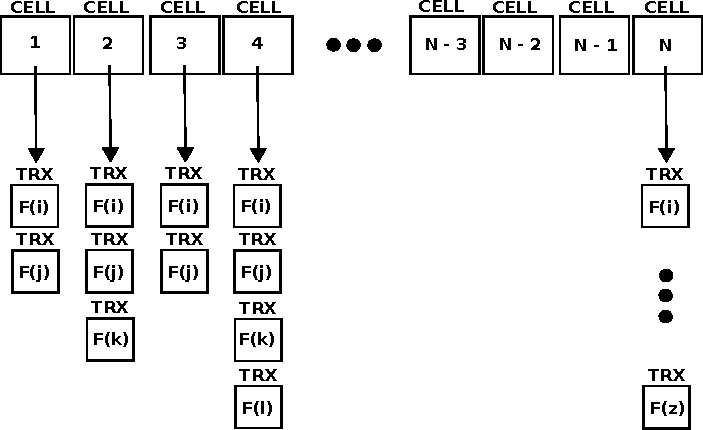
\includegraphics[width=4.8in, height=3.5in]{./pictures/fapPlanDiagram.pdf}}%
\lthtmlinlinemathZ
\lthtmlcheckvsize\clearpage}

{\newpage\clearpage
\lthtmlinlinemathA{tex2html_wrap_inline15613}%
$ N$%
\lthtmlinlinemathZ
\lthtmlcheckvsize\clearpage}

{\newpage\clearpage
\lthtmlinlinemathA{tex2html_wrap_inline15615}%
$ F(i)$%
\lthtmlinlinemathZ
\lthtmlcheckvsize\clearpage}

{\newpage\clearpage
\lthtmlfigureA{algorithm5516}%
\begin{algorithm}
% latex2html id marker 5516
[H]
\caption{The \gls{FAP} \gls{PSO} Algorithm}
\begin{algorithmic}
\State $s_n$\  = Initialize Swarm $s_n$
\While{Termination criterion not met}
	\State EvaluateSwarm($s_n$)
	\State UpdateGlobalBest($s_n$)
	\State UpdateSwarmMovement($s_n$,$gbest$)
\EndWhile
\end{algorithmic}
\end{algorithm}%
\lthtmlfigureZ
\lthtmlcheckvsize\clearpage}

\stepcounter{section}
{\newpage\clearpage
\lthtmlfigureA{algorithm5534}%
\begin{algorithm}
% latex2html id marker 5534

\caption{FAP Cost Function}
	\begin{algorithmic}[1]
	\Require normalCell
	\Require interferingCe;;
	\State $totalInterference \leftarrow $0
	\For{Each TRX $trx_i$\  in interferingCell}
		\For{Each TRX $trx_j$\  in normalCell}
			\State $interference \leftarrow 0$
			\State $difference \leftarrow$\  $|trx_i - trx_j|$
			\If{difference is 0}
				\If{coChannelInterference $\leq$\  minInterferenceThershold}
					\State $interference \leftarrow interference + 0$
				\Else
					\State $interference \leftarrow interference + coChannelInterference$
				\EndIf
			\Else
				\If{difference is 1}
					\If{adjChannelInterference $\leq$\  minInterferenceThershold}
						\State $interference \leftarrow interference + 0$
					\Else
						\State $interference \leftarrow interference + adjChannelInterference$
					\EndIf
				\EndIf
			\EndIf
			\State $totalInterference \leftarrow totalInterference + interference$
		\EndFor
	\EndFor
	\end{algorithmic}
\end{algorithm}%
\lthtmlfigureZ
\lthtmlcheckvsize\clearpage}

\stepcounter{section}
\stepcounter{subsection}
{\newpage\clearpage
\lthtmlinlinemathA{tex2html_wrap_inline15624}%
$ pbest - x_i(t)$%
\lthtmlinlinemathZ
\lthtmlcheckvsize\clearpage}

{\newpage\clearpage
\lthtmlinlinemathA{tex2html_wrap_inline15626}%
$ gbest - x_i(t)$%
\lthtmlinlinemathZ
\lthtmlcheckvsize\clearpage}

{\newpage\clearpage
\lthtmlinlinemathA{tex2html_wrap_inline15628}%
$ c_1\phi_1 * SubtractionResultPbest$%
\lthtmlinlinemathZ
\lthtmlcheckvsize\clearpage}

{\newpage\clearpage
\lthtmlinlinemathA{tex2html_wrap_inline15630}%
$ c_2\phi_2 * SubtractionResultGbest$%
\lthtmlinlinemathZ
\lthtmlcheckvsize\clearpage}

{\newpage\clearpage
\lthtmlinlinemathA{tex2html_wrap_inline15632}%
$ v_i(t) + MultiPbestResult + MultiGBestResult$%
\lthtmlinlinemathZ
\lthtmlcheckvsize\clearpage}

{\newpage\clearpage
\lthtmlfigureA{algorithm5572}%
\begin{algorithm}
% latex2html id marker 5572
[H]
\caption{Velocity Method 1}
	\begin{algorithmic}[1]
	\Require currentParticle
	\Require globalBestParticle
	\State $pbest \leftarrow $currentParticle position
	\State $gbest \leftarrow $globalBestParticle position
	\State $localCoeff \leftarrow getLocalCoefficient()$
	\State $globalCoeff \leftarrow getGlobalCoefficient()$
	\State $pBestSubtractResult \leftarrow $Subtract current Particle position from pbest
	\State $gBestSubtractResult \leftarrow $Subtract current Particle position from gbest
	\State $a \leftarrow $Multiply localCoeff with pBestSubtractResult and a random value
	\State $b \leftarrow $Multiply globalCoeff with gBestSubtractResult and a random value
	\If{first time velocity is calculated for current Particle}
		\State $currentParticle.Velocity \leftarrow $Add a and b
	\Else
		\State $abAdditionResult \leftarrow $Add a and b
		\State $inertia \leftarrow getInertia()$
		\State $newVelocity \leftarrow $Add abAdditionResult and currentParticle.Velocity
		\State $currentParticle.Velocity \leftarrow $Multiply inertia with newVelocity
	\EndIf
	\State $currentParticle.Position \leftarrow $Add currentParticle.Velocity and currentParticle.Position
	\State SanatizePosition(currentParticle.Position)
	\end{algorithmic}
\end{algorithm}%
\lthtmlfigureZ
\lthtmlcheckvsize\clearpage}

{\newpage\clearpage
\lthtmlfigureA{algorithm5581}%
\begin{algorithm}
% latex2html id marker 5581
[H]
\caption{Subtract One Position From Another} (Method 1)
\begin{algorithmic}[1]
	\Require fromPosition
	\Require toPosition
	\For{Each cell $c$\  in fromPosition}
		\For{Each transceiver $f_{trx}$\  in $c$}
			\State $t_{trx} \leftarrow$\  Get same $f_{trx}$\  in toPosition
			\State $f_{trx} \leftarrow f_{trx} - t_{trx}$
		\EndFor
	\EndFor
\end{algorithmic}
\end{algorithm}%
\lthtmlfigureZ
\lthtmlcheckvsize\clearpage}

{\newpage\clearpage
\lthtmlfigureA{algorithm5596}%
\begin{algorithm}
% latex2html id marker 5596
[H]
\caption{Multiply Position by a Value (Method 1)}
\begin{algorithmic}[1]
	\Require fromPosition
	\Require value
	\Require mustRandom
	\For{Each cell $c$\  in fromPosition}
		\For{Each transceiver $trx$\  in $c$}
			\If{must multiply with random number}
				\State $trx \leftarrow trx * value * random()$
			\Else
				\State $trx \leftarrow trx * value$
			\EndIf
		\EndFor
	\EndFor
\end{algorithmic}
\end{algorithm}%
\lthtmlfigureZ
\lthtmlcheckvsize\clearpage}

{\newpage\clearpage
\lthtmlinlinemathA{tex2html_wrap_inline15636}%
$ value$%
\lthtmlinlinemathZ
\lthtmlcheckvsize\clearpage}

{\newpage\clearpage
\lthtmlinlinemathA{tex2html_wrap_inline15638}%
$ 0.5 * v(t+1)$%
\lthtmlinlinemathZ
\lthtmlcheckvsize\clearpage}

{\newpage\clearpage
\lthtmlinlinemathA{tex2html_wrap_inline15640}%
$ v(t+1)$%
\lthtmlinlinemathZ
\lthtmlcheckvsize\clearpage}

{\newpage\clearpage
\lthtmlinlinemathA{tex2html_wrap_inline15648}%
$ \phi_1$%
\lthtmlinlinemathZ
\lthtmlcheckvsize\clearpage}

{\newpage\clearpage
\lthtmlinlinemathA{tex2html_wrap_inline15650}%
$ \phi_2$%
\lthtmlinlinemathZ
\lthtmlcheckvsize\clearpage}

{\newpage\clearpage
\lthtmlfigureA{algorithm5616}%
\begin{algorithm}
% latex2html id marker 5616
[H]
\caption{Add One Position to Another (Method 1)}
\begin{algorithmic}[1]
	\Require fromPosition
	\Require toPosition
	\For{Each cell $c$\  in fromPosition}
		\For{Each transceiver $f_{trx}$\  in $c$}
			\State $t_{trx} \leftarrow$\  Get same $f_{trx}$\  in toPosition
			\State $f_{trx} \leftarrow f_{trx} + t_{trx}$
			\State Bound($t_{trx}$)
		\EndFor
	\EndFor
\end{algorithmic}
\end{algorithm}%
\lthtmlfigureZ
\lthtmlcheckvsize\clearpage}

\stepcounter{subsection}
{\newpage\clearpage
\lthtmlfigureA{algorithm5639}%
\begin{algorithm}
% latex2html id marker 5639
[H]
\caption{BoundValue Method}
\begin{algorithmic}[1]
	\Require Position
	\For{Each cell $c_i$\  in Position}
		\For{Each transceiver $trx_j$\  in $c_i$}
			\State $trx_j = \left|trx_j\right|$
			\If{$trx_j \geq maxChannelValue$}
				\State $trx_j = minChannelValue + (\text{$trx_j$\  mod $maxChannelValue$})$
			\Else 
				\If{$trx_j \leq minChannelValue$}
					\State BoundValue($trx_j + minChannelValue$)
				\EndIf
			\EndIf
		\EndFor
	\EndFor
\end{algorithmic}
\end{algorithm}%
\lthtmlfigureZ
\lthtmlcheckvsize\clearpage}

{\newpage\clearpage
\lthtmlinlinemathA{tex2html_wrap_indisplay15656}%
$\displaystyle 10 mod 50 =$%
\lthtmlindisplaymathZ
\lthtmlcheckvsize\clearpage}

{\newpage\clearpage
\lthtmlinlinemathA{tex2html_wrap_indisplay15657}%
$\displaystyle 10$%
\lthtmlindisplaymathZ
\lthtmlcheckvsize\clearpage}

{\newpage\clearpage
\lthtmlinlinemathA{tex2html_wrap_indisplay15658}%
$\displaystyle 60 mod 50 =$%
\lthtmlindisplaymathZ
\lthtmlcheckvsize\clearpage}

{\newpage\clearpage
\lthtmlinlinemathA{tex2html_wrap_indisplay15660}%
$\displaystyle 50 mod 50 =$%
\lthtmlindisplaymathZ
\lthtmlcheckvsize\clearpage}

{\newpage\clearpage
\lthtmlinlinemathA{tex2html_wrap_indisplay15661}%
$\displaystyle 100 mod 50 =$%
\lthtmlindisplaymathZ
\lthtmlcheckvsize\clearpage}

{\newpage\clearpage
\lthtmlinlinemathA{tex2html_wrap_indisplay15662}%
$\displaystyle 35 mod 50 =$%
\lthtmlindisplaymathZ
\lthtmlcheckvsize\clearpage}

{\newpage\clearpage
\lthtmlinlinemathA{tex2html_wrap_indisplay15663}%
$\displaystyle 35$%
\lthtmlindisplaymathZ
\lthtmlcheckvsize\clearpage}

{\newpage\clearpage
\lthtmlinlinemathA{tex2html_wrap_inline15665}%
$ [0,50]$%
\lthtmlinlinemathZ
\lthtmlcheckvsize\clearpage}

\stepcounter{subsection}
{\newpage\clearpage
\lthtmlfigureA{algorithm5676}%
\begin{algorithm}
% latex2html id marker 5676
[H]
\caption{Velocity Method 2}
\begin{algorithmic}[1]
	\Require currentParticle
	\Require globalBestParticle
	\State $currPos \leftarrow$\  currentParticle position
	\State $pbestPos \leftarrow$\  currentParticle best position
	\State $gbestPos \leftarrow$\  global best particle position
	\For{Each cell $c$\  in $currPos$}
		\State $c_{pbestPos} \leftarrow $\  Same cell in $pbestPos$
		\State $c_{gbestPos} \leftarrow $\  Same cell in $gbestPos$
		\State $movedIndices \leftarrow $MoveIndices($c_{pbestPos},c,c_{gbestPos}$)
		\If{First time velocity is calculated}
			\State ApplyVelocity(c,movedIndices)
		\Else
			\State $newVelocity \leftarrow CalculateIndexVelocity(currPos.velocity,movedIndices)$
			\State ApplyVelocity(c,newVelocity)
		\EndIf
	\EndFor
	\State SanatizePosition(currPos)
\end{algorithmic}
\end{algorithm}%
\lthtmlfigureZ
\lthtmlcheckvsize\clearpage}

{\newpage\clearpage
\lthtmlinlinemathA{tex2html_wrap_inline15672}%
$ pbestPos$%
\lthtmlinlinemathZ
\lthtmlcheckvsize\clearpage}

{\newpage\clearpage
\lthtmlinlinemathA{tex2html_wrap_inline15674}%
$ gbestPos$%
\lthtmlinlinemathZ
\lthtmlcheckvsize\clearpage}

{\newpage\clearpage
\lthtmlfigureA{algorithm5690}%
\begin{algorithm}
% latex2html id marker 5690

\caption{MoveIndices}
\begin{algorithmic}[1]
	\Require pbestCell
	\Require currCell
	\Require gbestCell
	\For{Each $trx_i$\  in currCell}
		\State $pbestTRX_i$\  = Get $trx_i$\  in pbestCell
		\State $gbestTRX_i$\  = Get $trx_i$\  in gbestCell
		\State $r1 \leftarrow$\  Random double number
		\State $r2 \leftarrow$\  Random double number
		\State $localCoeff \leftarrow getLocalCoefficient()$
		\State $globalCoeff \leftarrow getGlobalCoefficient()$
		\State $a \leftarrow localCoef * r1 * (pbestTRX_i - trx_i)$
		\State $b \leftarrow globalCoef * r2 * (pbestTRX_i - gbestTRX_i)$
		\State $trx_i \leftarrow a + b$
	\EndFor
\end{algorithmic}
\end{algorithm}%
\lthtmlfigureZ
\lthtmlcheckvsize\clearpage}

{\newpage\clearpage
\lthtmlfigureA{algorithm5704}%
\begin{algorithm}
% latex2html id marker 5704

\caption{ApplyVelocity}
\begin{algorithmic}[1]
	\Require currPos
	\Require velocity
	\For{Each index $c_i$\  in currPos}
		\State $c_i \leftarrow c_i + velocity_i$
	\EndFor
\end{algorithmic}
\end{algorithm}%
\lthtmlfigureZ
\lthtmlcheckvsize\clearpage}

{\newpage\clearpage
\lthtmlfigureA{algorithm5717}%
\begin{algorithm}
% latex2html id marker 5717

\caption{CalculateIndexVelocity}
\begin{algorithmic}[1]
	\Require currVelocity
	\Require newVelocity
	\For{Each value $v_i$\  in currVelocity}
		\State $inertia \leftarrow getInertia()$
		\State $v_i \leftarrow v_i + (inertia * newVelocity_i)$
	\EndFor
\end{algorithmic}
\end{algorithm}%
\lthtmlfigureZ
\lthtmlcheckvsize\clearpage}

\stepcounter{section}
{\newpage\clearpage
\lthtmlfigureA{algorithm5736}%
\begin{algorithm}
% latex2html id marker 5736

\caption{Standard Gbest Selection in \gls{FAP} \gls{PSO} }
\begin{algorithmic}[1]
\Require swarm
\Require gbest
\State $gbestCost$\  = Evaluate(gbest)
\For{Each particle $p_i$\  in swarm}
	\State $cost$\  = Evaluate($p_i$)
	\If{$cost \leq gbestCost$}
		\State $gbestCost = cost$
		\State gbest = $p_i$
	\EndIf
\EndFor
\Return gbest
\end{algorithmic}
\end{algorithm}%
\lthtmlfigureZ
\lthtmlcheckvsize\clearpage}

{\newpage\clearpage
\lthtmlfigureA{algorithm5781}%
\begin{algorithm}
% latex2html id marker 5781
[H]
\caption{Building Global Best with Cells}
\begin{algorithmic}[1]
\Require gbest
\Require swarm
\For{Each particle $p_i$\  in swarm}
	\For{Each cell $c_j$\  in $p_i$}
		\State $gbestcell_j$\  = Get cell $c_j$\  in gbest
		\State $cellCost$\  = Get total interference for cell $c_j$
		\State $gbestCellCost$\  = Get total interference for cell $gbestcell_j$
		\If{$cellCost \leq gbestCellCost$}
			\State $gbestcell_j$\  = $c_j$
		\EndIf
	\EndFor
\EndFor
\end{algorithmic}
\end{algorithm}%
\lthtmlfigureZ
\lthtmlcheckvsize\clearpage}

{\newpage\clearpage
\lthtmlfigureA{algorithm5790}%
\begin{algorithm}
% latex2html id marker 5790
[H]
\caption{Building Global Best with Transceivers}
\begin{algorithmic}[1]
\Require gbest
\Require swarm
\For{Each particle $p_i$\  in swarm}
	\For{Each cell $c_j$\  in $p_i$}
		\For{Each transceiver $trx_k$\  in $c_j$}
			\State $gbestTrx_k$\  = Get $trx_k$\  in $c_j$\  in gbest
			\State $trxCost$\  = Get total interference for $trx_k$
			\State $gbestTrxCost$\  = Get total interference for cell $gbestTrx_j$
			\If{$trxCost \leq gbestTrxCost$}
				\State $gbestTrx_k$\  = $trx_k$
			\EndIf
		\EndFor
	\EndFor
\EndFor
\end{algorithmic}
\end{algorithm}%
\lthtmlfigureZ
\lthtmlcheckvsize\clearpage}

{\newpage\clearpage
\lthtmlinlinemathA{tex2html_wrap_inline15681}%
$ c_j$%
\lthtmlinlinemathZ
\lthtmlcheckvsize\clearpage}

\stepcounter{section}
{\newpage\clearpage
\lthtmlfigureA{algorithm5833}%
\begin{algorithm}
% latex2html id marker 5833
[H]
\caption{SanitizePosition}
\begin{algorithmic}[1]
	\Require currPosition
	\For{Each cell $c_i$\  in currPosition}
		\State $tbList = $\  Get Tabu List of currPosition
		\State ResolveCollision($c_i$,$tbList$)
		\State AdhereToSeparation($c_i$)
	\EndFor
\end{algorithmic}
\end{algorithm}%
\lthtmlfigureZ
\lthtmlcheckvsize\clearpage}

{\newpage\clearpage
\lthtmlfigureA{algorithm5846}%
\begin{algorithm}
% latex2html id marker 5846
[H]
\caption{ResolveCollision}
\begin{algorithmic}[1]
	\Require cell
	\Require tabuList
	\For{Each $trx_i$\  in cell}
			\While{$trx_i$\  exists in TabuList}
				\State $trx_i = $\  Generate random frequency
				\If{Collision not resolved after 20 attempts}
					\State Break out of while loop
				\EndIf
			\EndWhile
	\EndFor
\end{algorithmic}
\end{algorithm}%
\lthtmlfigureZ
\lthtmlcheckvsize\clearpage}

\stepcounter{section}
\stepcounter{chapter}
\stepcounter{section}
\stepcounter{section}
\stepcounter{subsection}
\stepcounter{subsection}
\stepcounter{subsection}
\stepcounter{subsection}
\stepcounter{subsection}
\stepcounter{section}
\stepcounter{subsection}
\stepcounter{subsection}
\stepcounter{subsection}
\stepcounter{section}
\stepcounter{chapter}
\stepcounter{section}
\stepcounter{section}
\stepcounter{section}
\stepcounter{section}
\stepcounter{subsection}
\stepcounter{subsubsection}
\stepcounter{subsubsection}
\stepcounter{subsubsection}
\stepcounter{subsubsection}
\stepcounter{subsubsection}
\stepcounter{subsection}
\stepcounter{subsubsection}
\stepcounter{subsubsection}
\stepcounter{subsubsection}
\stepcounter{subsection}
\stepcounter{section}

\end{document}
